\documentclass[aspectratio=43]{beamer}
% \documentclass[aspectratio=169]{beamer}

% Title --------------------------------------------
\title[Lecture 5: Advanced topics]{\Large Advanced topics \& overview}
\author[]{Francisco Villamil}
\date[]{Research Design for Social Sciences\\MA Computational Social Science, UC3M\\Fall 2023}

%%% NOTE -- CHECK THIS: https://github.com/paulgp/beamer-tips


%%% Building heavily on https://github.com/kylebutts/templates

% xcolor, define them
\usepackage{xcolor}

% TEXT COLORS
\definecolor{red}{HTML}{9a2515}
\definecolor{yellow}{HTML}{EBC944}
\definecolor{asher}{HTML}{555F61}
\definecolor{jet}{HTML}{131516}

% THEME COLORS
\definecolor{accent}{HTML}{107895}
\definecolor{accent2}{HTML}{9a2515}

% Color commands
\newcommand\red[1]{{\color{red}#1}}
\newcommand\yellow[1]{{\color{yellow}#1}}
\newcommand\asher[1]{{\color{asher}#1}}

\newcommand\BGred[1]{{\colorbox{red!80!white}{#1}}}
\newcommand\BGyellow[1]{{\colorbox{yellow!80!white}{#1}}}
\newcommand\BGasher[1]{{\colorbox{asher!80!white}{#1}}}

% Appendix numbering
\usepackage{appendixnumberbeamer}

% Beamer Options -------------------------------------

% Background
\setbeamercolor{background canvas}{bg = white}

% Change text margins
\setbeamersize{text margin left = 25pt, text margin right = 15pt}

% \alert
\setbeamercolor{alerted text}{fg = accent2}

% Frame title
\setbeamercolor{frametitle}{bg = white, fg = jet}
\setbeamercolor{framesubtitle}{bg = white, fg = accent}
\setbeamerfont{framesubtitle}{size = \small, shape = \itshape}

% Block
\setbeamercolor{block title}{fg = white, bg = accent2}
\setbeamercolor{block body}{fg = jet, bg = jet!10!white}

% Title page
\setbeamercolor{title}{fg = jet}
\setbeamercolor{subtitle}{fg = accent}

%% Custom \maketitle and \titlepage
\setbeamertemplate{title page}
{
    \begin{centering}
      % \vspace{20mm}
      {\Large \usebeamerfont{title}\usebeamercolor[fg]{title}\inserttitle}\\ \vskip0.25em%
      \ifx\insertsubtitle\@empty%
      \else%
        {\usebeamerfont{subtitle}\usebeamercolor[fg]{subtitle}\insertsubtitle\par}%
      \fi%
      {\vspace{10mm}\insertauthor}\\
      \ifx\insertinstitute\@empty%
      \else%
        {\vspace{5mm}\color{asher}\scriptsize{\insertinstitute}}\\\vspace{5mm}
      \fi%
      {\color{asher}\small{\insertdate}}\\
    \end{centering}
}

% Table of Contents
\setbeamercolor{section in toc}{fg = accent!70!jet}
\setbeamercolor{subsection in toc}{fg = jet}

% Button
\setbeamercolor{button}{bg = accent}

% Remove navigation symbols
\setbeamertemplate{navigation symbols}{}

% Table and Figure captions
\setbeamercolor{caption}{fg=jet!70!white}
\setbeamercolor{caption name}{fg=jet}
\setbeamerfont{caption name}{shape = \itshape}

% Put slide number / total slides at the bottom right
\makeatother
\makeatletter
\setbeamertemplate{footline} %{\hfill\insertframenumber/\inserttotalframenumber}
{%
  \leavevmode%
  \hbox{
  \begin{beamercolorbox}[wd=\paperwidth,ht=2.5ex,dp=1.125ex,leftskip=.3cm,rightskip=.3cm plus1fil]{footlinecolor}%
    \color{asher}{{\let\hyperlink\@secondoftwo\insertshorttitle}\hfill\insertshortauthor\hfill\insertshortdate\hfill\insertframenumber/\inserttotalframenumber}
  \end{beamercolorbox}}%
  \vskip0pt%
}
\makeatother
\makeatletter

% Bullet points

%% Fix left-margins
\settowidth{\leftmargini}{\usebeamertemplate{itemize item}}
\addtolength{\leftmargini}{\labelsep}

%% enumerate item color
\setbeamercolor{enumerate item}{fg = accent}
\setbeamerfont{enumerate item}{size = \small}
\setbeamertemplate{enumerate item}{\insertenumlabel.}

%% itemize
\setbeamercolor{itemize item}{fg = accent!70!white}
\setbeamerfont{itemize item}{size = \small}
\setbeamertemplate{itemize item}[circle]
\setlength{\itemsep}{0pt plus 6pt}

%% right arrow for subitems
\setbeamercolor{itemize subitem}{fg = accent!60!white}
\setbeamerfont{itemize subitem}{size = \small}
\setbeamertemplate{itemize subitem}{$\rightarrow$}

\setbeamertemplate{itemize subsubitem}[square]
\setbeamercolor{itemize subsubitem}{fg = jet}
\setbeamerfont{itemize subsubitem}{size = \small}

% References

%% Bibliography Font, roughly matching aea
\setbeamerfont{bibliography item}{size = \footnotesize}
\setbeamerfont{bibliography entry author}{size = \footnotesize, series = \bfseries}
\setbeamerfont{bibliography entry title}{size = \footnotesize}
\setbeamerfont{bibliography entry location}{size = \footnotesize, shape = \itshape}
\setbeamerfont{bibliography entry note}{size = \footnotesize}

\setbeamercolor{bibliography item}{fg = jet}
\setbeamercolor{bibliography entry author}{fg = accent!60!jet}
\setbeamercolor{bibliography entry title}{fg = jet}
\setbeamercolor{bibliography entry location}{fg = jet}
\setbeamercolor{bibliography entry note}{fg = jet}

%% Remove bibliography symbol in slides
\setbeamertemplate{bibliography item}{}





% Links ----------------------------------------------

\usepackage{hyperref}
\hypersetup{
  colorlinks = true,
  linkcolor = accent2,
  filecolor = accent2,
  urlcolor = accent2,
  citecolor = accent2,
}


% Line spacing --------------------------------------
\usepackage{setspace}
\setstretch{1.2}


% \begin{columns} -----------------------------------
\usepackage{multicol}


% % Fonts ---------------------------------------------
% % Beamer Option to use custom fonts
% \usefonttheme{professionalfonts}
%
% % \usepackage[utopia, smallerops, varg]{newtxmath}
% % \usepackage{utopia}
% \usepackage[sfdefault,light]{roboto}
%
% % Small adjustments to text kerning
% \usepackage{microtype}



% Remove annoying over-full box warnings -----------
\vfuzz2pt
\hfuzz2pt


% Table of Contents with Sections
\setbeamerfont{myTOC}{series=\bfseries, size=\Large}
\AtBeginSection[]{
        \frame{
            \frametitle{Roadmap}
            \tableofcontents[current]
        }
    }


% References ----------------------------------------
\usepackage[
    citestyle= authoryear,
    style = authoryear,
    natbib = true,
    backend = biber
]{biblatex}

% Smaller font-size for references
\renewcommand*{\bibfont}{\small}

% Remove "In:"
\renewbibmacro{in:}{}

% Color citations for slides
\newenvironment{citecolor}
    {\footnotesize\begin{color}{accent2}}
    {\end{color}}

\newcommand{\citetcolor}[1]{{\footnotesize\textcolor{asher}{\citet{#1}}}}
\newcommand{\citepcolor}[1]{{\footnotesize\textcolor{asher}{\citep{#1}}}}

% Tables -------------------------------------------
% Tables too big
% \begin{adjustbox}{width = 1.2\textwidth, center}
\usepackage{adjustbox}
\usepackage{array}
\usepackage{threeparttable, booktabs, adjustbox}

% Fix \input with tables
% \input fails when \\ is at end of external .tex file

\makeatletter
\let\input\@@input
\makeatother

% Tables too narrow
% \begin{tabularx}{\linewidth}{cols}
% col-types: X - center, L - left, R -right
% Relative scale: >{\hsize=.8\hsize}X/L/R
\usepackage{tabularx}
\newcolumntype{L}{>{\raggedright\arraybackslash}X}
\newcolumntype{R}{>{\raggedleft\arraybackslash}X}
\newcolumntype{C}{>{\centering\arraybackslash}X}

% Figures

% \imageframe{img_name} -----------------------------
% from https://github.com/mattjetwell/cousteau
\newcommand{\imageframe}[1]{%
    \begin{frame}[plain]
        \begin{tikzpicture}[remember picture, overlay]
            \node[at = (current page.center), xshift = 0cm] (cover) {%
                \includegraphics[keepaspectratio, width=\paperwidth, height=\paperheight]{#1}
            };
        \end{tikzpicture}
    \end{frame}%
}

% subfigures
\usepackage{subfigure}


% Highlight slide -----------------------------------
% \begin{transitionframe} Text \end{transitionframe}
% from paulgp's beamer tips
\newenvironment{transitionframe}{
    \setbeamercolor{background canvas}{bg=accent!60!black}
    \begin{frame}\color{accent!10!white}\LARGE\centering
}{
    \end{frame}
}


% Table Highlighting --------------------------------
% Create top-left and bottom-right markets in tabular cells with a unique matching id and these commands will outline those cells
\usepackage[beamer,customcolors]{hf-tikz}
\usetikzlibrary{calc}
\usetikzlibrary{fit,shapes.misc}

% To set the hypothesis highlighting boxes red.
\newcommand\marktopleft[1]{%
    \tikz[overlay,remember picture]
        \node (marker-#1-a) at (0,1.5ex) {};%
}
\newcommand\markbottomright[1]{%
    \tikz[overlay,remember picture]
        \node (marker-#1-b) at (0,0) {};%
    \tikz[accent!80!jet, ultra thick, overlay, remember picture, inner sep=4pt]
        \node[draw, rectangle, fit=(marker-#1-a.center) (marker-#1-b.center)] {};%
}


\begin{document}
% ====================================================

% ----------------------------------------------------
\begin{frame}
  \titlepage
\end{frame}
% ----------------------------------------------------

\section{Generalizing results}

% ----------------------------------------------------
\begin{frame}
\frametitle{Generalizing results}
\centering

\begin{itemize}
  \item The \BGyellow{Credibility Revolution} in social sciences
  \item What are we really learning?
  \item References:
  \begin{itemize}
    \item Egami and Hartman (2023) \href{https://doi.org/10.1017/S0003055422000880}{Elements of External Validity: Framework, Design, and Analysis}. \textit{APSR} 117(3): 1070--1088.
    \item Munger (2023) \href{https://doi.org/10.1177/20531680231187271}{Temporal validity as meta-science}. \textit{Res\&Pol} 10(3).
    \begin{itemize}
      \item See also this post: \href{https://kevinmunger.substack.com/p/generalizing-knowledge-of-twitter}{Generalizing Knowledge of Twitter to ``X''}.
    \end{itemize}
    \item Esterling, Brady, \& Schwitzgebel (2023) \href{https://osf.io/2s8w5/}{The Necessity of Construct and External Validity for Generalized Causal Claims: A Critical Review of the Literature on Quantitative Causal Inference}. Preprint.
  \end{itemize}
\end{itemize}

\end{frame}
% ----------------------------------------------------

% ----------------------------------------------------
\begin{frame}
\frametitle{Generalizing results}
\centering

\begin{itemize}
  \item \BGyellow{Construct validity}: are we really measuring what we intent to?
  \begin{itemize}
    \item is the treatment doing what we theoretically expect it to? and are we measuring the outcome correctly?
  \end{itemize}
  \item \BGyellow{External validity}: would we get the same results if we replicate this in another context?
  \begin{itemize}
    \item especially: temporal and spatial validity
  \end{itemize}
\end{itemize}

\end{frame}
% ----------------------------------------------------

\section{Robustness and inference tests}


% ----------------------------------------------------
\begin{frame}
\frametitle{Basic guidelines on robustness tests}
\centering



\end{frame}
% ----------------------------------------------------

% ----------------------------------------------------
\begin{frame}
\frametitle{Inference tests: placebo tests}
\centering

\begin{itemize}
  \item Reference:
  \begin{itemize}
    \item AC Eggers, G Tuñón, A Dafoe (2023) \href{https://doi.org/10.1111/ajps.12818}{Placebo Tests for Causal Inference}. \textit{American Journal of Political Science}, published online.
  \end{itemize}
\end{itemize}

\end{frame}
% ----------------------------------------------------

\section{Mechanism test and additional implications}

% ----------------------------------------------------
\begin{frame}
\frametitle{Testing the mechanism}
\centering



\end{frame}
% ----------------------------------------------------

% ----------------------------------------------------
\begin{frame}
\frametitle{Additional implications of the theory}
\centering



\end{frame}
% ----------------------------------------------------

\section{Causal methods in detail}


\subsection{Controlling and matching}

% ----------------------------------------------------
\begin{frame}
\frametitle{Controlling in regression}
\centering

\begin{itemize}
  \item We probably already know this
  \item We've seen what it means controlling: just adjusting for the variation already predicted by the other variables
  \item One limitation though: we need to \textit{observe} those variables
\end{itemize}

\end{frame}
% ----------------------------------------------------

% ----------------------------------------------------
\begin{frame}
\frametitle{Controlling}
\centering

\begin{itemize}
  \item We are going to see two further methods of controlling widely used:
  \begin{itemize}
    \item Matching
    \item Fixed effects
  \end{itemize}
\end{itemize}

\end{frame}
% ----------------------------------------------------

% ----------------------------------------------------
\begin{frame}
\frametitle{Matching}
\centering

\begin{itemize}
  \item Adding control variables is not the only way to control / close back doors
  \item Imagine we have the following model:
  \begin{itemize}
    \item Z $\rightarrow$ X {\color{red}{$\rightarrow$}} Y $\leftarrow$ Z
    \item Where $Z$ is whether someone is retired or not
  \end{itemize}
  \item If we select a sample of \textit{only} retired people, we are closing that back door
  \begin{itemize}
    \item (X $\leftarrow$ Z $\rightarrow$ Y)
  \end{itemize}
  \item Matching is something like this, it's basically about creating groups of comparison where $Z$ (which can be several variables) does not vary
\end{itemize}

\end{frame}
% ----------------------------------------------------

% ----------------------------------------------------
\begin{frame}
\frametitle{How matching works}
\centering

\begin{itemize}
  \item We have a treatment group and a control group (so: \textit{binary} treatment variables)
  \item The main idea: give different \textit{weights} to treated and control observations, so we eliminate
  \item We get these weights by using one or more \textit{matching variables} (i.e. confounding variables)
\end{itemize}

\end{frame}
% ----------------------------------------------------

% ----------------------------------------------------
\begin{frame}
\frametitle{How matching works}
\centering

\begin{itemize}
  \item Imagine we have:
  \begin{itemize}
    \item Treatment: get some specific skill training
    \item Outcome: jet a job afterwards
    \item Confounding variable: gender
  \end{itemize}
  \item Control group: 80 men and 20 women
  \begin{itemize}
    \item 75\% of men get a job, 60\% of women do
  \end{itemize}
  \item Treatment group: 500 men and 500 women
  \begin{itemize}
    \item 70\% of men get a job, 55\% of women do
  \end{itemize}
  \item Comparing within each group, we know the treatment effect is a 5\% increase in the odds of getting a job (70 $\rightarrow$ 75, 55 $\rightarrow$ 60)
  \item But if we do the global comparison, it's almost 10\%
    \begin{itemize}
      \item 60 men + 12 women out of 100 = $72/100 = 72\%$, vs $(350+275)/1000 = 62.5\%$, so a difference of 9.5 points
    \end{itemize}
  \end{itemize}

\end{frame}
% ----------------------------------------------------

% ----------------------------------------------------
\begin{frame}
\frametitle{How matching works}
\centering

\begin{itemize}
  \item The problem is we have 4 times more men in the treated group than women, whereas we have equal proportion on the control group
  \item So we'll weight the control observations by gender, giving \textit{more} weight to the men observations, so it looks more similar to the treatment group
  \item $(4 * 350 + 1 * 275) / (4 * 500 + 1 * 500) = 67\%$
  \item Now, the unweighted difference in the treatment group was 72\%, and now the weighted difference in the control group is 67\%
  \item The difference is 5 points, the same as the within-group calculation we did before
\end{itemize}

\end{frame}
% ----------------------------------------------------

% ----------------------------------------------------
\begin{frame}
\frametitle{Two approaches to matching}
\centering

\begin{itemize}
  \item[1.] \textbf{Distance matching}
  \begin{itemize}
    \item We want to create a dataset where treatment and control observations have similar values (distance) in the confounding variables
    \item If, say, our confounding variable is income, we'll pick control observations that have a similar value on income to each of the treatment observations
    \item \href{https://nickchk.com/causalgraphs.html}{{https://nickchk.com/causalgraphs.html}}
  \end{itemize}
\end{itemize}

\uncover<4->{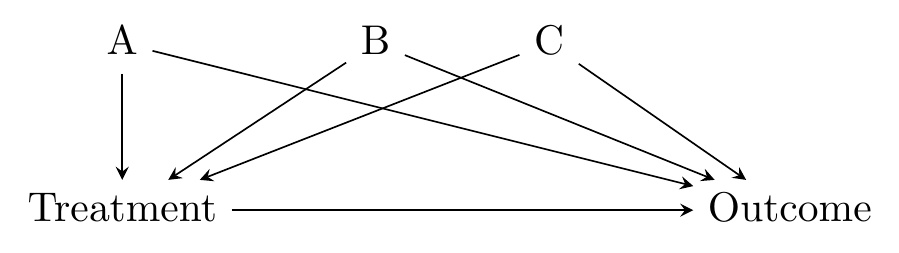
\includegraphics[width = 0.8\textwidth]{../img/matching_dag_distance}}

\end{frame}
% ----------------------------------------------------

% ----------------------------------------------------
\begin{frame}
\frametitle{Two approaches to matching}
\centering

\begin{itemize}
  \item[2.] \textbf{Propensity score matching}
  \begin{itemize}
    \item We want to account for the differential likelihood in getting into treatment depending on the value of the confounding variables
    \item We estimate the probability of getting into treatment, usually by doing a regression where the outcome is the treatment and the right-hand variables are the confounders
    \item We control for the propensity score matching, or select based on it (or both)
  \end{itemize}
\end{itemize}

\uncover<4->{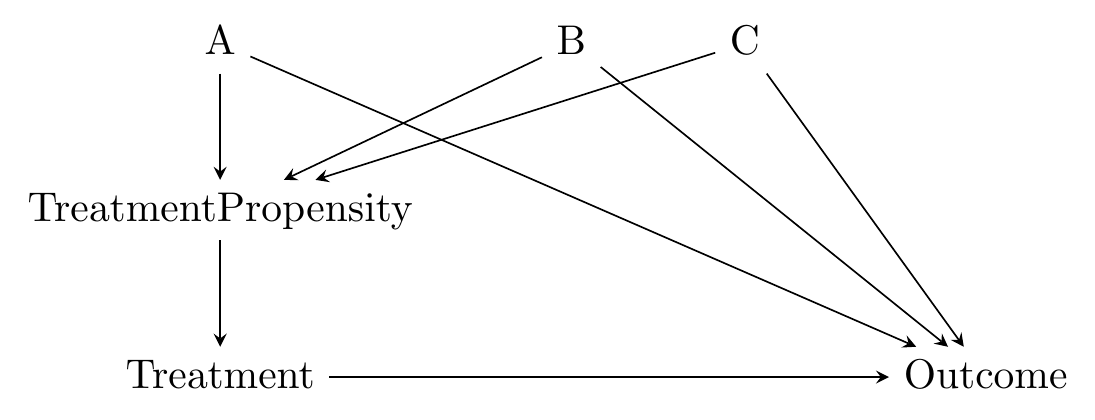
\includegraphics[width = \textwidth]{../img/matching_dag_ps}}

\end{frame}
% ----------------------------------------------------

% ----------------------------------------------------
\begin{frame}
\frametitle{Two approaches to matching: propensity score}
\centering

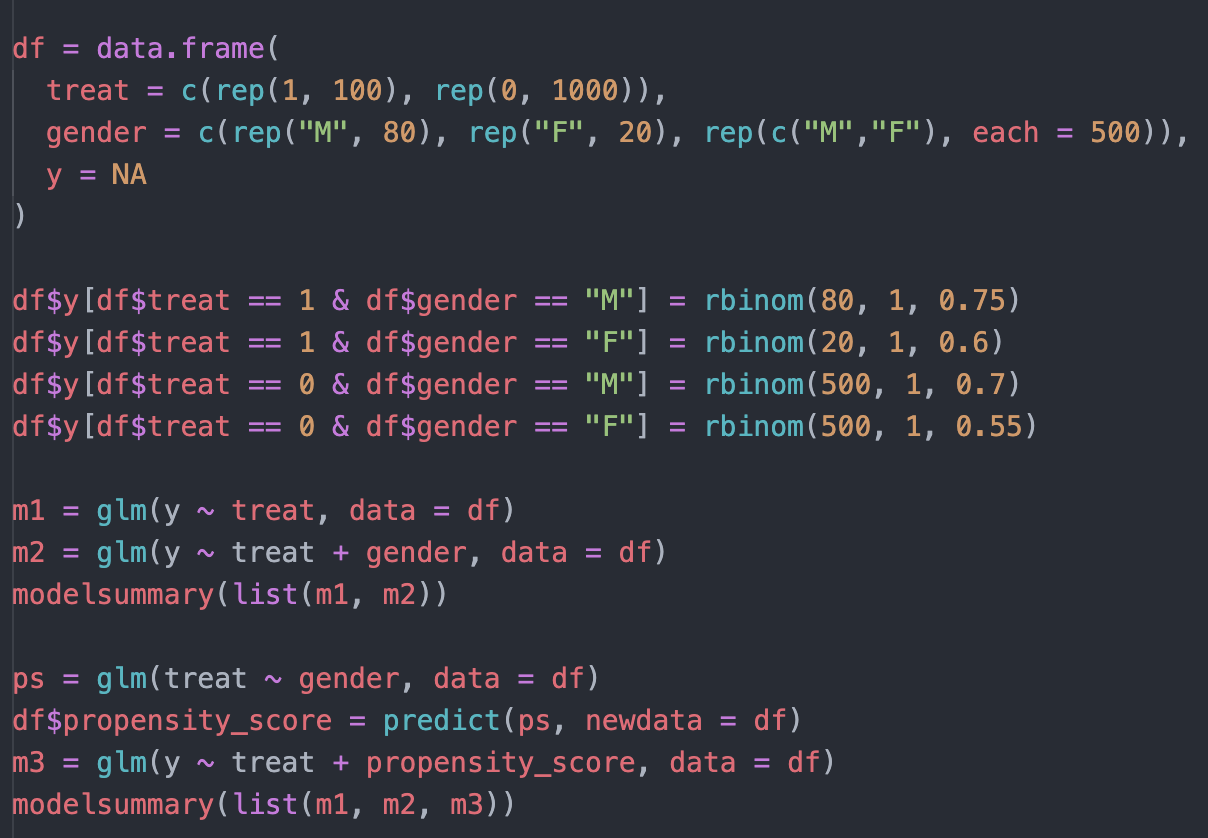
\includegraphics[width = \textwidth]{../img/propscore1}

\end{frame}
% ----------------------------------------------------

% ----------------------------------------------------
\begin{frame}
\frametitle{Two approaches to matching: propensity score}
\centering

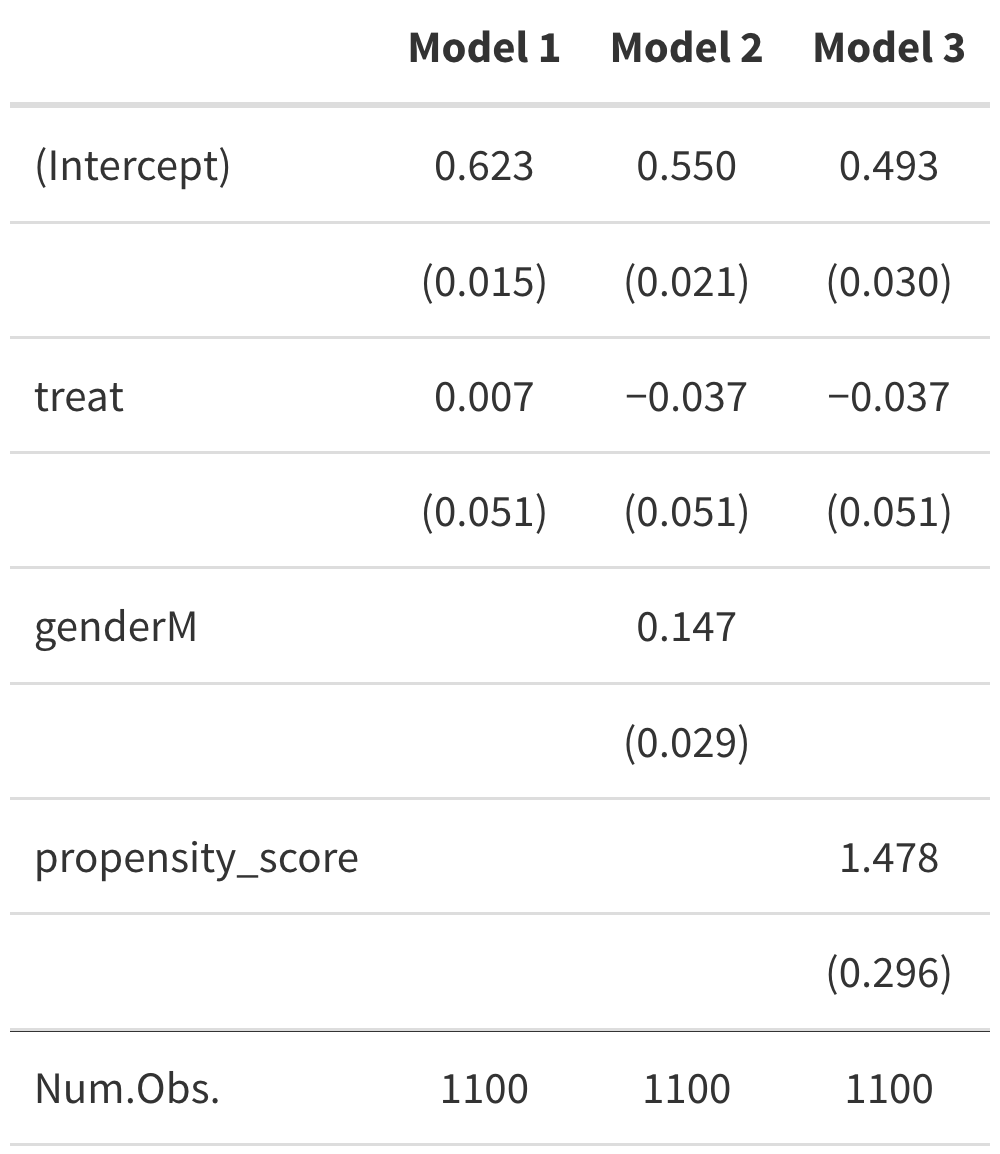
\includegraphics[width = 0.6\textwidth]{../img/propscore2}

\end{frame}
% ----------------------------------------------------

% ----------------------------------------------------
\begin{frame}
\frametitle{Matching vs regression}
\centering

\begin{itemize}
  \item Matching and regression are complementary approaches
  \item e.g. regression doesn't waste any information, but has a linearity assumption
  \item It's usual to use both at the same time
\end{itemize}

\end{frame}
% ----------------------------------------------------

\subsection{Fixed effects}

% ----------------------------------------------------
\begin{frame}
\frametitle{Fixed effects}
\centering

\begin{itemize}
  \item The problem with covariate adjustment, regardless of whether we use regression or matching, is that we need to \textit{observe} those variables
  \item But another strategy when we have unobserved confounders is to try within-group comparisons, which will work when the unobserved variance is contact within some group
  \item For example, imagine cases when our $U$ variable is:
  \begin{itemize}
    \item \textit{Country history}, in a cross-national analysis
    \item \textit{City of origin}, in an individual-level analysis
    \item \textit{Individual background}, in a panel survey analysis
    \item \textit{Company effects}, if we look at the effects of English courses on internal promotion using individual data from many different companies
    \item etc
  \end{itemize}
\end{itemize}

\end{frame}
% ----------------------------------------------------

% ----------------------------------------------------
\begin{frame}
\frametitle{Fixed effects - when do we use them?}
\centering

\begin{tikzpicture}
% nodes %
\node (Y) at (2,0){Outcome};
\node (D) at (-2,0){Treatment};
\node (U) at (0,3){U};
\draw[->] (D) -- (Y);
\draw[->, dashed] (U) -- (D);
\draw[->, dashed] (U) -- (Y);
\end{tikzpicture}

\end{frame}
% ----------------------------------------------------

% ----------------------------------------------------
\begin{frame}
\frametitle{Fixed effects - when do we use them?}
\centering

\begin{tikzpicture}
% nodes %
\node (Y) at (2,0){BA 1st year grades};
\node (D) at (-2,0){High School grades};
\node (U1) at (-2,3){Private HS's inflation};
\node (U2) at (0,4){Annoyed teachers};
\node (U3) at (2,5){Class environ};
\draw[->] (D) -- (Y);
\draw[->, dashed] (U1) -- (D);
\draw[->, dashed] (U1) -- (Y);
\draw[->, dashed] (U2) -- (D);
\draw[->, dashed] (U2) -- (Y);
\draw[->, dashed] (U3) -- (D);
\draw[->, dashed] (U3) -- (Y);
\end{tikzpicture}

\end{frame}
% ----------------------------------------------------

% ----------------------------------------------------
\begin{frame}
\frametitle{Fixed effects}
\centering

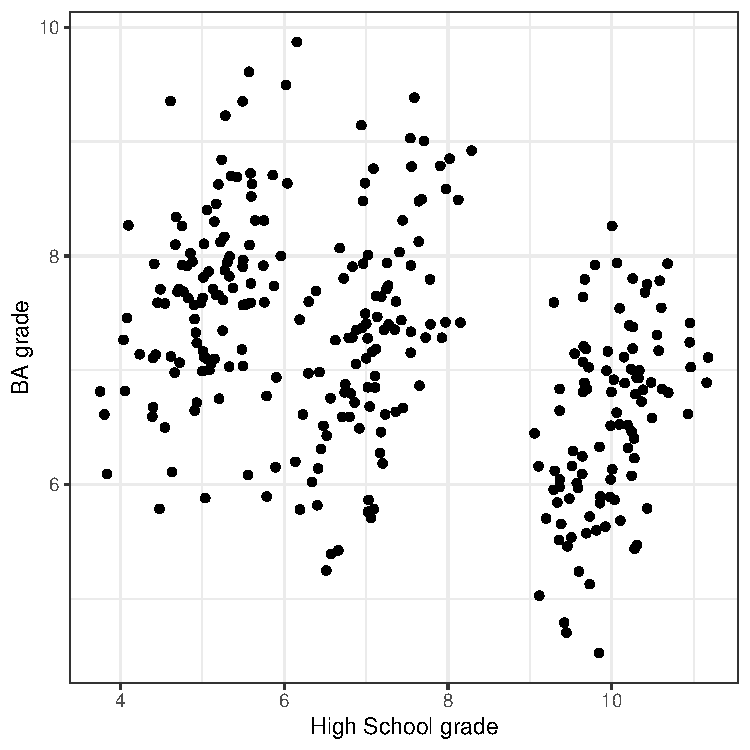
\includegraphics[width = 0.75\textwidth]{../img/fe1}

\end{frame}
% ----------------------------------------------------

% ----------------------------------------------------
\begin{frame}
\frametitle{Fixed effects}
\centering

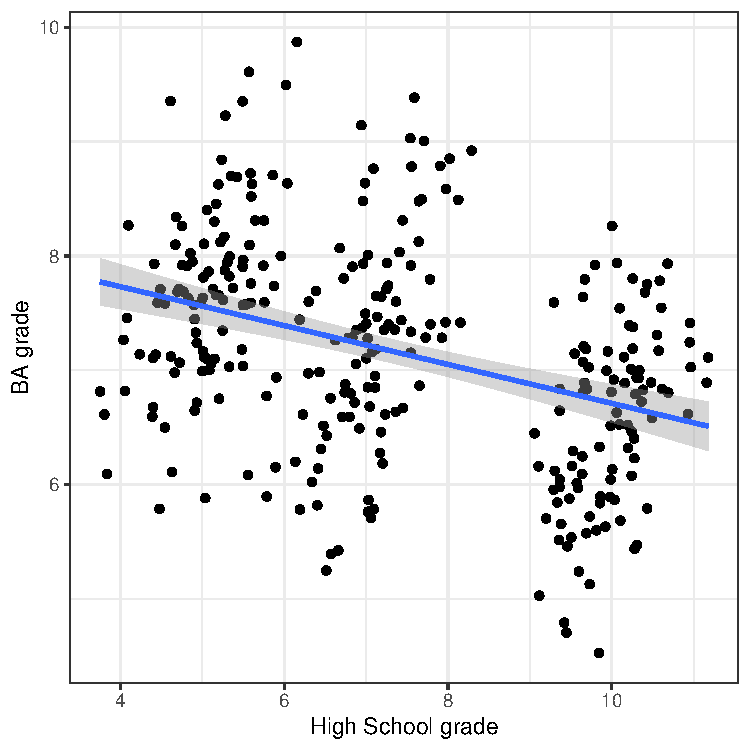
\includegraphics[width = 0.75\textwidth]{../img/fe2}

\end{frame}
% ----------------------------------------------------

% ----------------------------------------------------
\begin{frame}
\frametitle{Fixed effects}
\centering

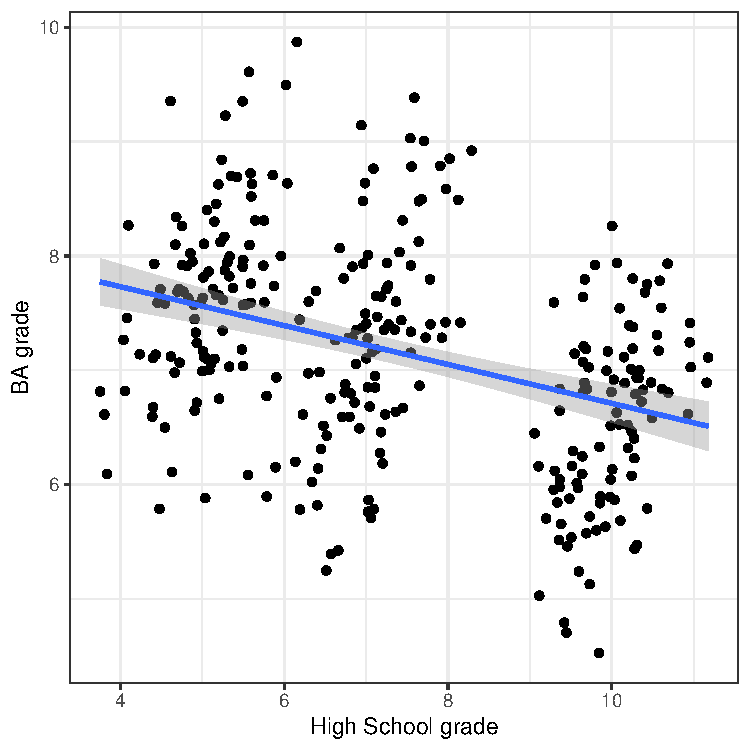
\includegraphics[width = 0.75\textwidth]{../img/fe2}

\end{frame}
% ----------------------------------------------------

% ----------------------------------------------------
\begin{frame}
\frametitle{Fixed effects}
\centering

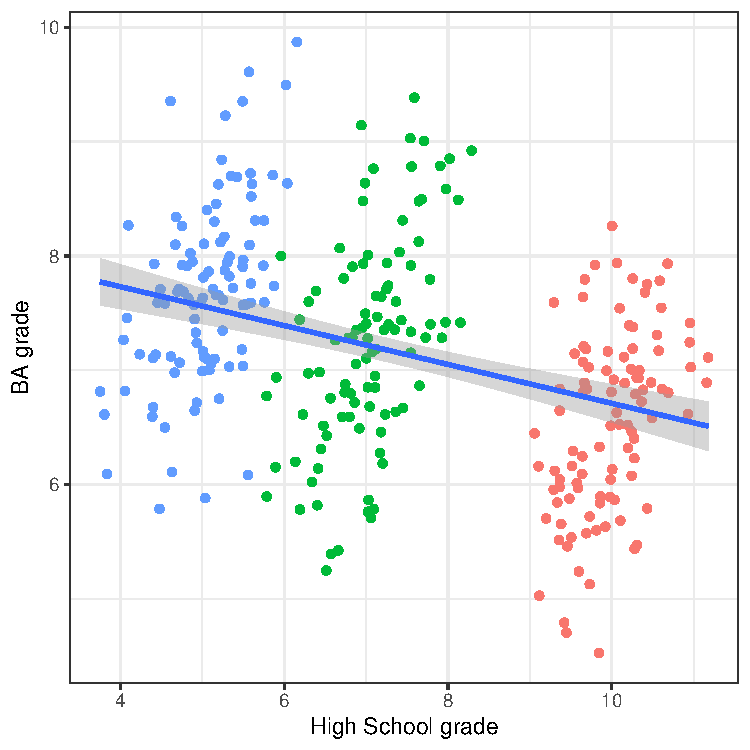
\includegraphics[width = 0.75\textwidth]{../img/fe3}

\end{frame}
% ----------------------------------------------------

% ----------------------------------------------------
\begin{frame}
\frametitle{Fixed effects}
\centering

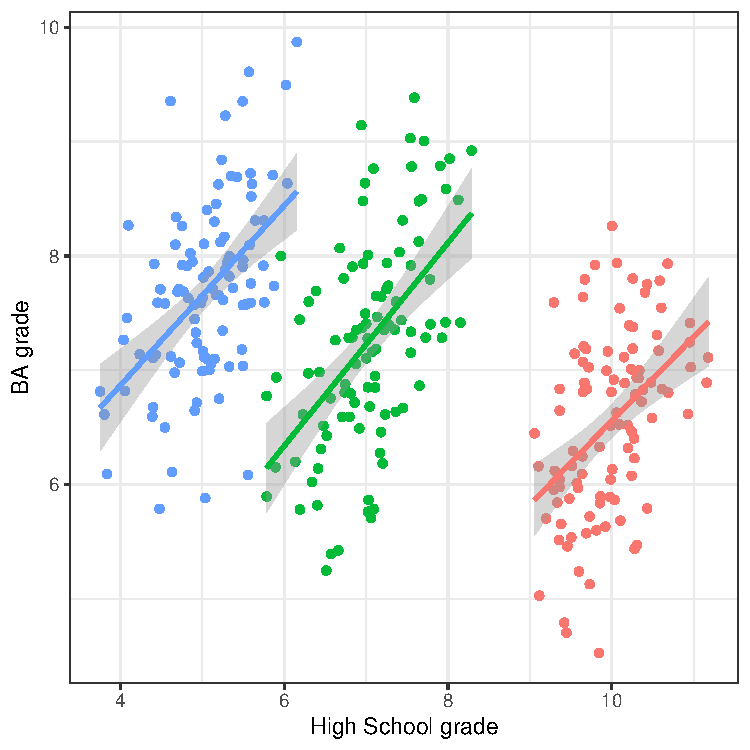
\includegraphics[width = 0.75\textwidth]{../img/fe4}

\end{frame}
% ----------------------------------------------------

% ----------------------------------------------------
\begin{frame}
\frametitle{Fixed effects}
\centering

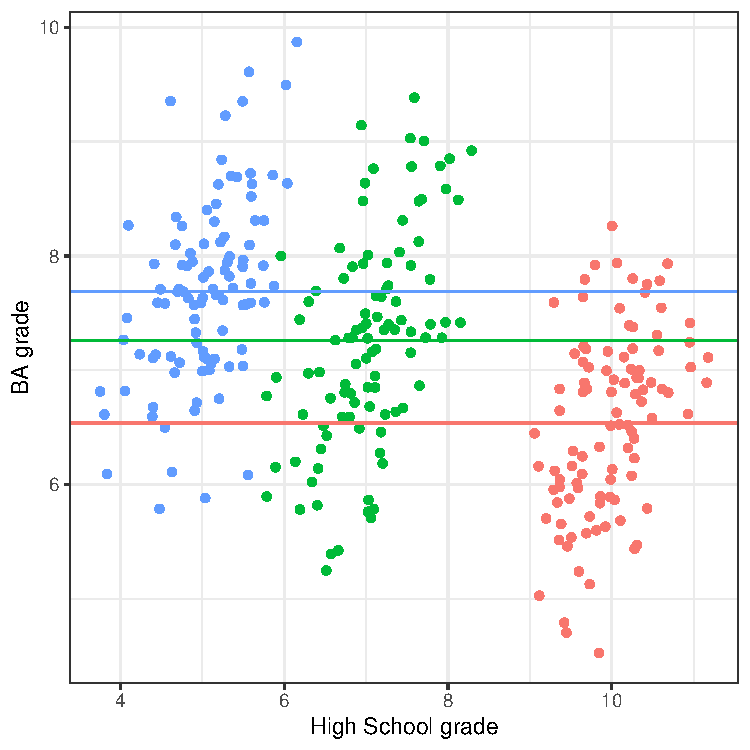
\includegraphics[width = 0.75\textwidth]{../img/fe5}

\end{frame}
% ----------------------------------------------------

% ----------------------------------------------------
\begin{frame}
\frametitle{Fixed effects}
\centering

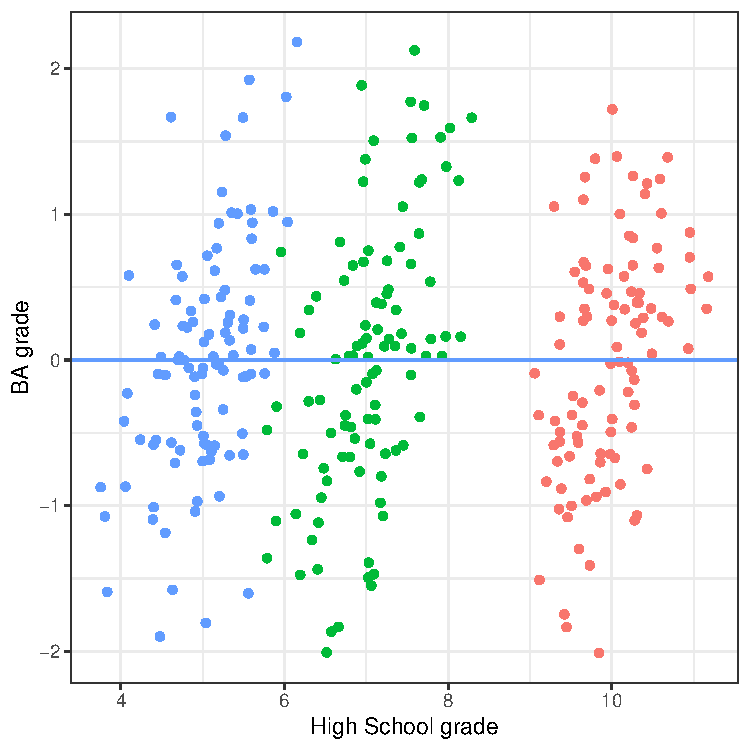
\includegraphics[width = 0.75\textwidth]{../img/fe6}

\end{frame}
% ----------------------------------------------------

% ----------------------------------------------------
\begin{frame}
\frametitle{Fixed effects}
\centering

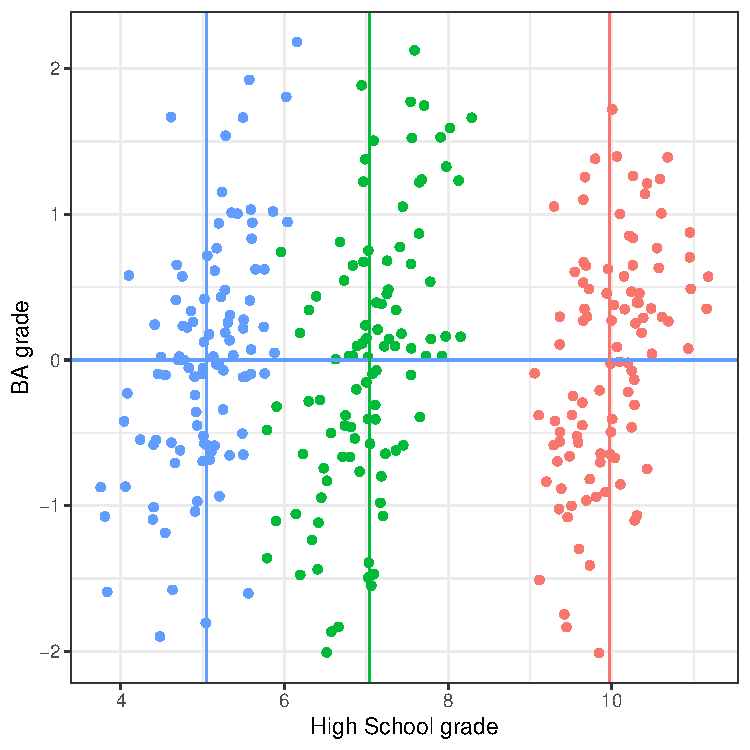
\includegraphics[width = 0.75\textwidth]{../img/fe7}

\end{frame}
% ----------------------------------------------------

% ----------------------------------------------------
\begin{frame}
\frametitle{Fixed effects}
\centering

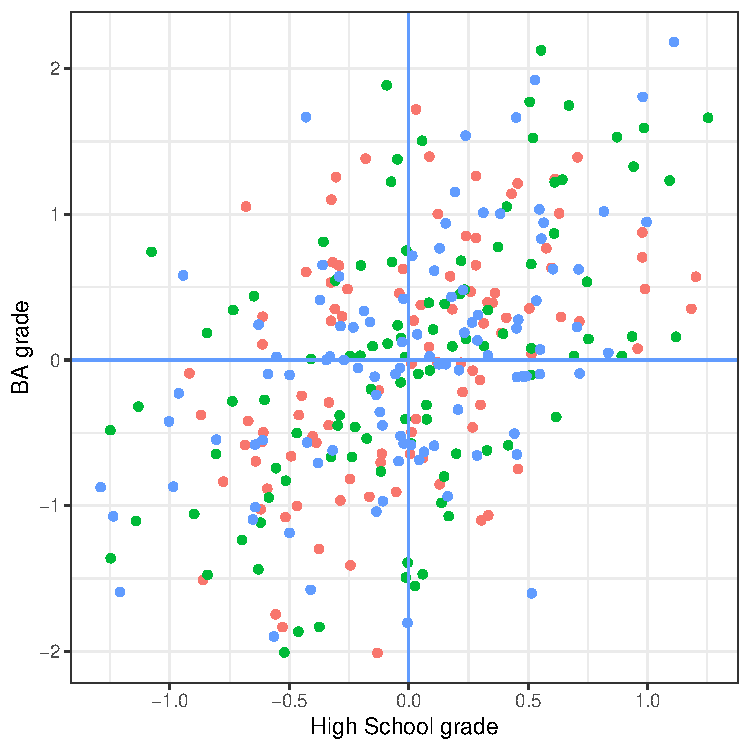
\includegraphics[width = 0.75\textwidth]{../img/fe8}

\end{frame}
% ----------------------------------------------------

% ----------------------------------------------------
\begin{frame}
\frametitle{Fixed effects}
\centering

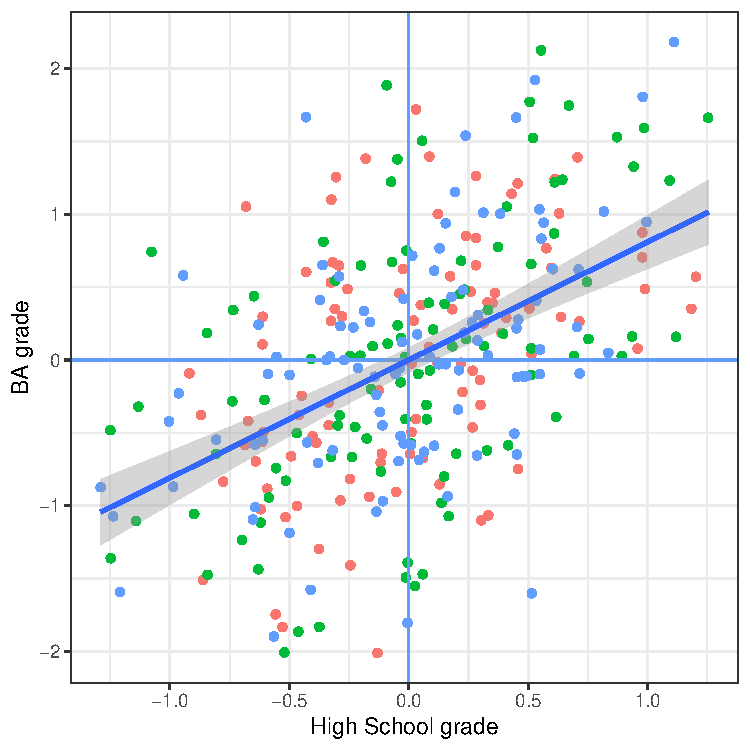
\includegraphics[width = 0.75\textwidth]{../img/fe9}

\end{frame}
% ----------------------------------------------------

% ----------------------------------------------------
\begin{frame}
\frametitle{Fixed effects and regression}
\centering

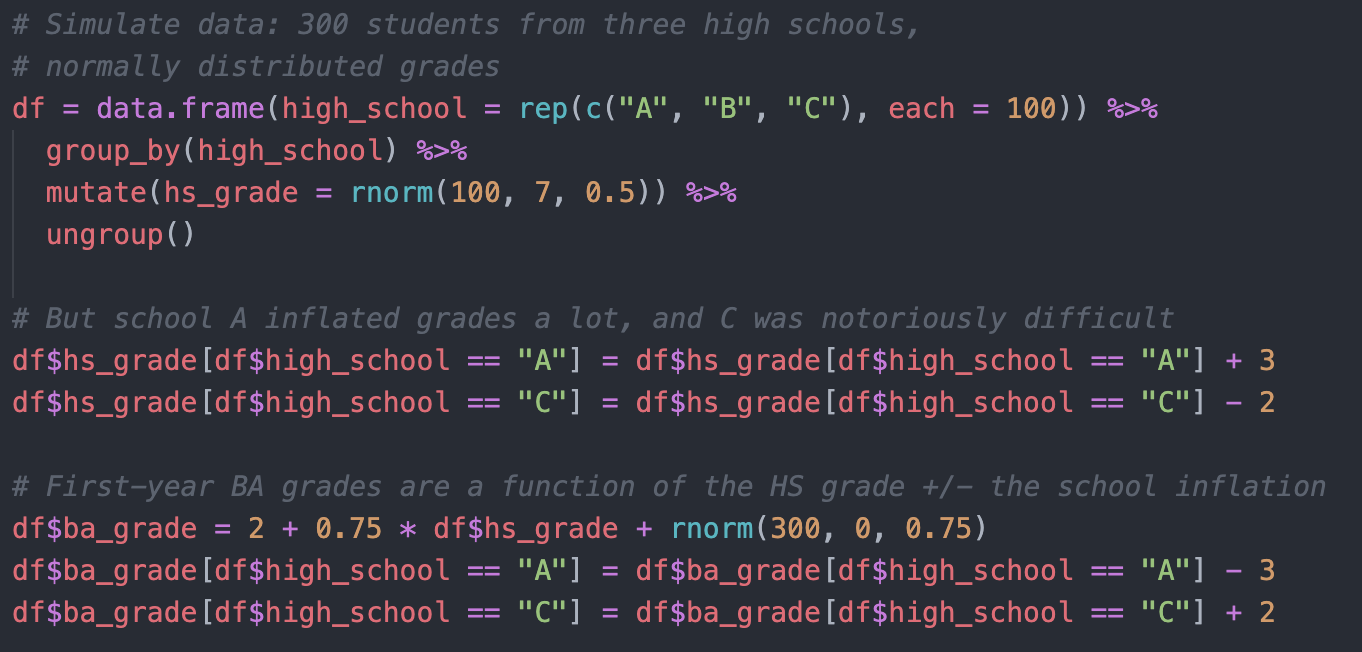
\includegraphics[width = \textwidth]{../img/fe_data}

Our true causal model

\end{frame}
% ----------------------------------------------------

% ----------------------------------------------------
\begin{frame}
\frametitle{Fixed effects and regression}
\centering

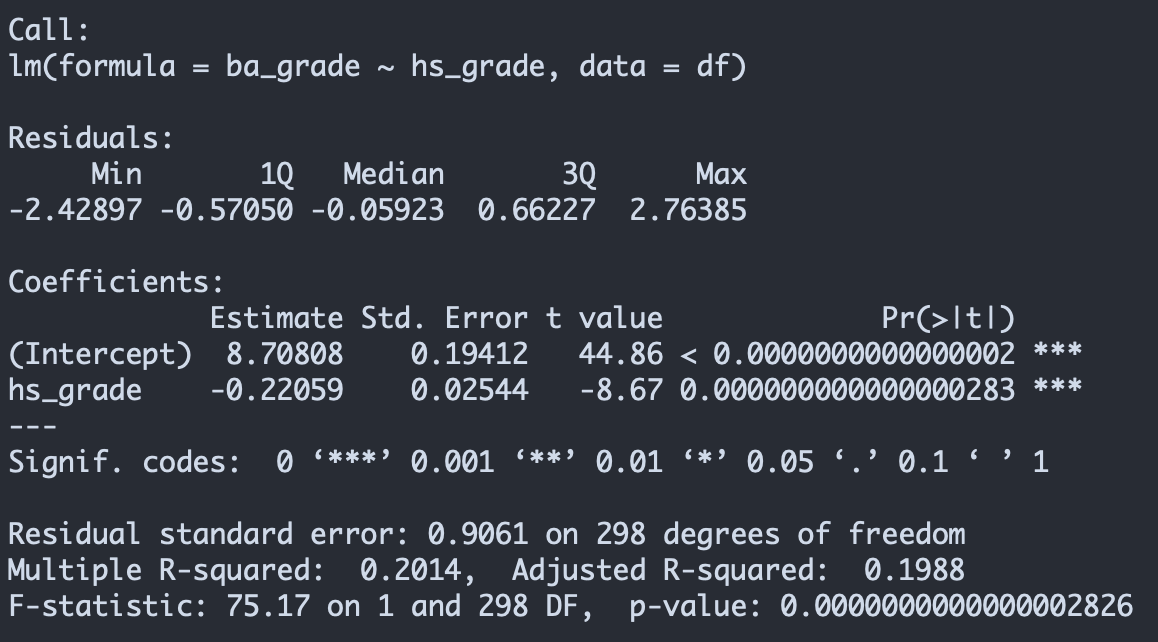
\includegraphics[width = \textwidth]{../img/fe_lm1}

\end{frame}
% ----------------------------------------------------

% ----------------------------------------------------
\begin{frame}
\frametitle{Fixed effects and regression}
\centering

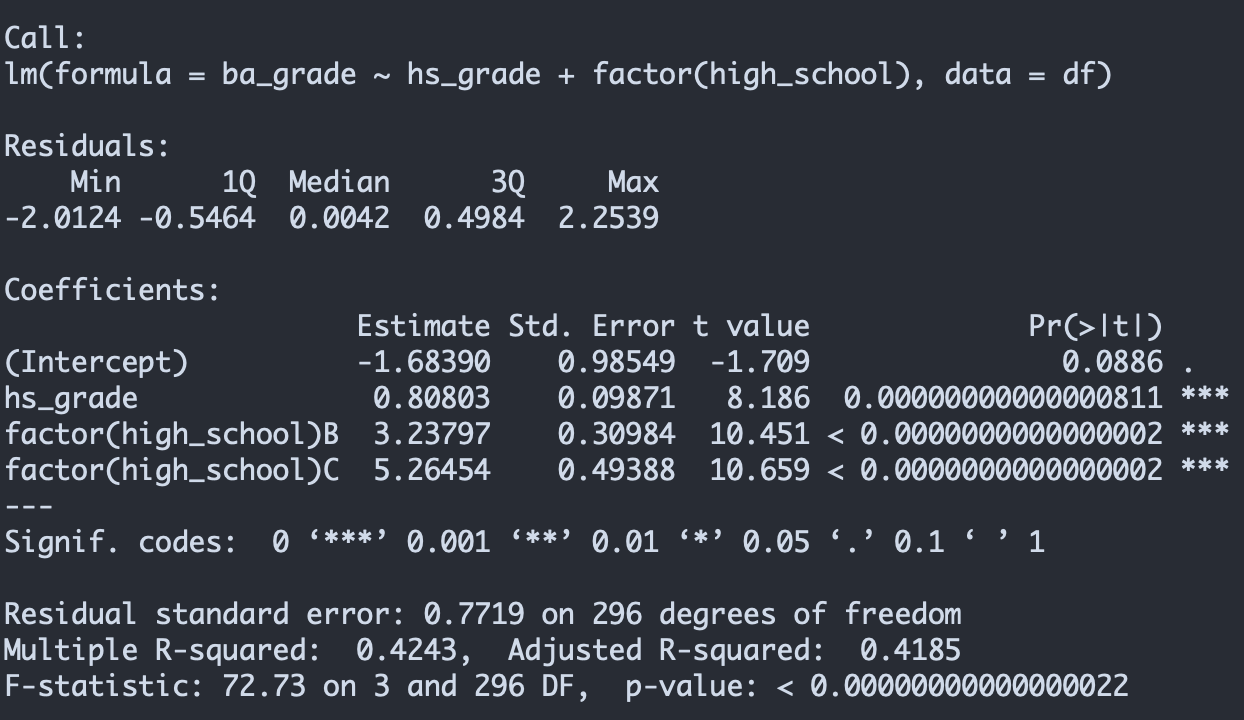
\includegraphics[width = \textwidth]{../img/fe_lm2}

\end{frame}
% ----------------------------------------------------

\subsection{Difference-in-differences}

% ----------------------------------------------------
\begin{frame}
\frametitle{Difference-in-differences}
\centering

\begin{itemize}
  \item Treatments usually occur at a particular moment in time, e.g.:
  \begin{itemize}
    \item Minimum wage increase
    \item Terrorist attack
    \item Influx of refugees
    \item ...
  \end{itemize}
  \item In those cases, if we have before \& after observations, we have something like this:
\end{itemize}

\begin{tikzpicture}
% nodes %
\node (Y) at (2,0){Outcome};
\node (D) at (-2,0){Treatment};
\node (U) at (0,1){Time};
\draw[->] (D) -- (Y);
\draw[->] (U) -- (D);
\draw[->] (U) -- (Y);
\end{tikzpicture}

\begin{itemize}
  \item The \textbf{problem} is that \textbf{all} the variation goes through time, so if we close that back door, we're left with nothing
\end{itemize}

\end{frame}
% ----------------------------------------------------

% ----------------------------------------------------
\begin{frame}
\frametitle{Difference-in-differences}
\centering

\begin{itemize}
  \item So one strategy we can use is to bring additional group that is \textit{not treated} and for which we also have before/after observations
  \begin{itemize}
    \item Minimum wage increase: maybe those earning above MW?
    \item Influx of refugees: other countries? regions far from the border?
    \item Terrorist attack: do we have a control (untreated) group?
    \item ...
  \end{itemize}
\end{itemize}

\begin{tikzpicture}
% nodes %
\node (Y) at (2,0){Outcome};
\node (D) at (-2,0){Treatment};
\node (U) at (0,1){Time};
\node (G) at (0,-1){Group};
\draw[->] (D) -- (Y);
\draw[->] (U) -- (D);
\draw[->] (U) -- (Y);
\draw[->] (G) -- (Y);
\draw[->] (G) -- (D);
\end{tikzpicture}

\end{frame}
% ----------------------------------------------------

% ----------------------------------------------------
\begin{frame}
\frametitle{Difference-in-differences}
\centering

\begin{tikzpicture}
% nodes %
\node (Y) at (2,0){Outcome};
\node (D) at (-2,0){Treatment};
\node (U) at (0,1){Time};
\node (G) at (0,-1){Group};
\draw[->] (D) -- (Y);
\draw[->] (U) -- (D);
\draw[->] (U) -- (Y);
\draw[->] (G) -- (Y);
\draw[->] (G) -- (D);
\end{tikzpicture}

\begin{itemize}
  \item We can compare changes across time \textit{within} the treated and control groups (closing the back door through \texttt{group})
  \item Compare within-group variation between treated and control (since time affects both `within-variations' the same way, we are closign the other back door through \texttt{time})
\end{itemize}

\end{frame}
% ----------------------------------------------------

% ----------------------------------------------------
\begin{frame}
\frametitle{Difference-in-differences}
\centering

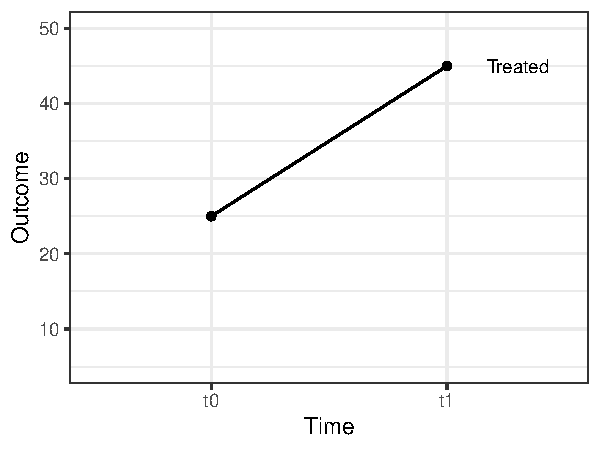
\includegraphics[width = 0.8\textwidth]{../img/did1}

\end{frame}
% ----------------------------------------------------

% ----------------------------------------------------
\begin{frame}
\frametitle{Difference-in-differences}
\centering

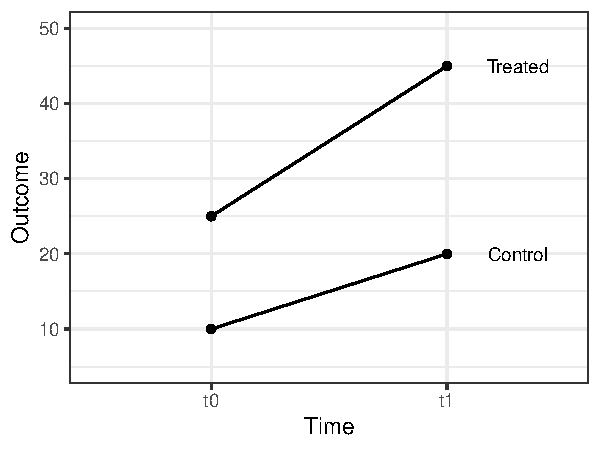
\includegraphics[width = 0.8\textwidth]{../img/did2}

\end{frame}
% ----------------------------------------------------

% ----------------------------------------------------
\begin{frame}
\frametitle{Difference-in-differences}
\centering

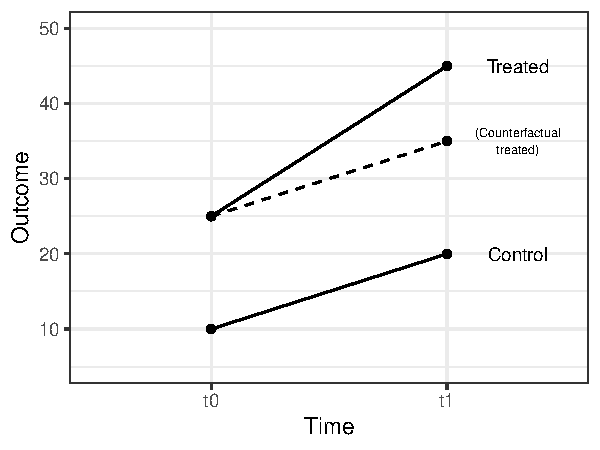
\includegraphics[width = 0.8\textwidth]{../img/did3}

\end{frame}
% ----------------------------------------------------

% ----------------------------------------------------
\begin{frame}
\frametitle{Difference-in-differences}
\centering

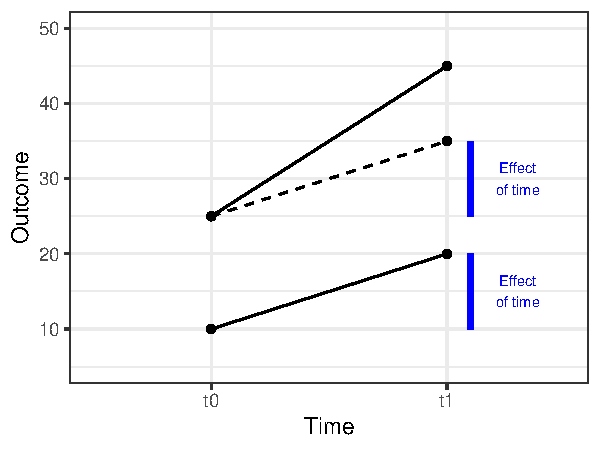
\includegraphics[width = 0.8\textwidth]{../img/did4}

\end{frame}
% ----------------------------------------------------

% ----------------------------------------------------
\begin{frame}
\frametitle{Difference-in-differences}
\centering

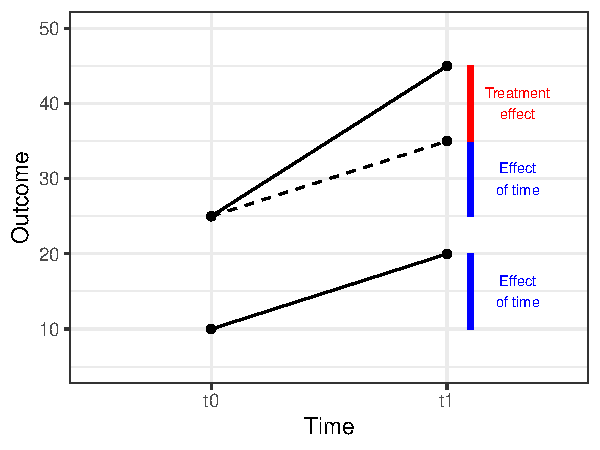
\includegraphics[width = 0.8\textwidth]{../img/did5}

\end{frame}
% ----------------------------------------------------

% ----------------------------------------------------
\begin{frame}
\frametitle{Difference-in-differences: Cholera in London}
\centering

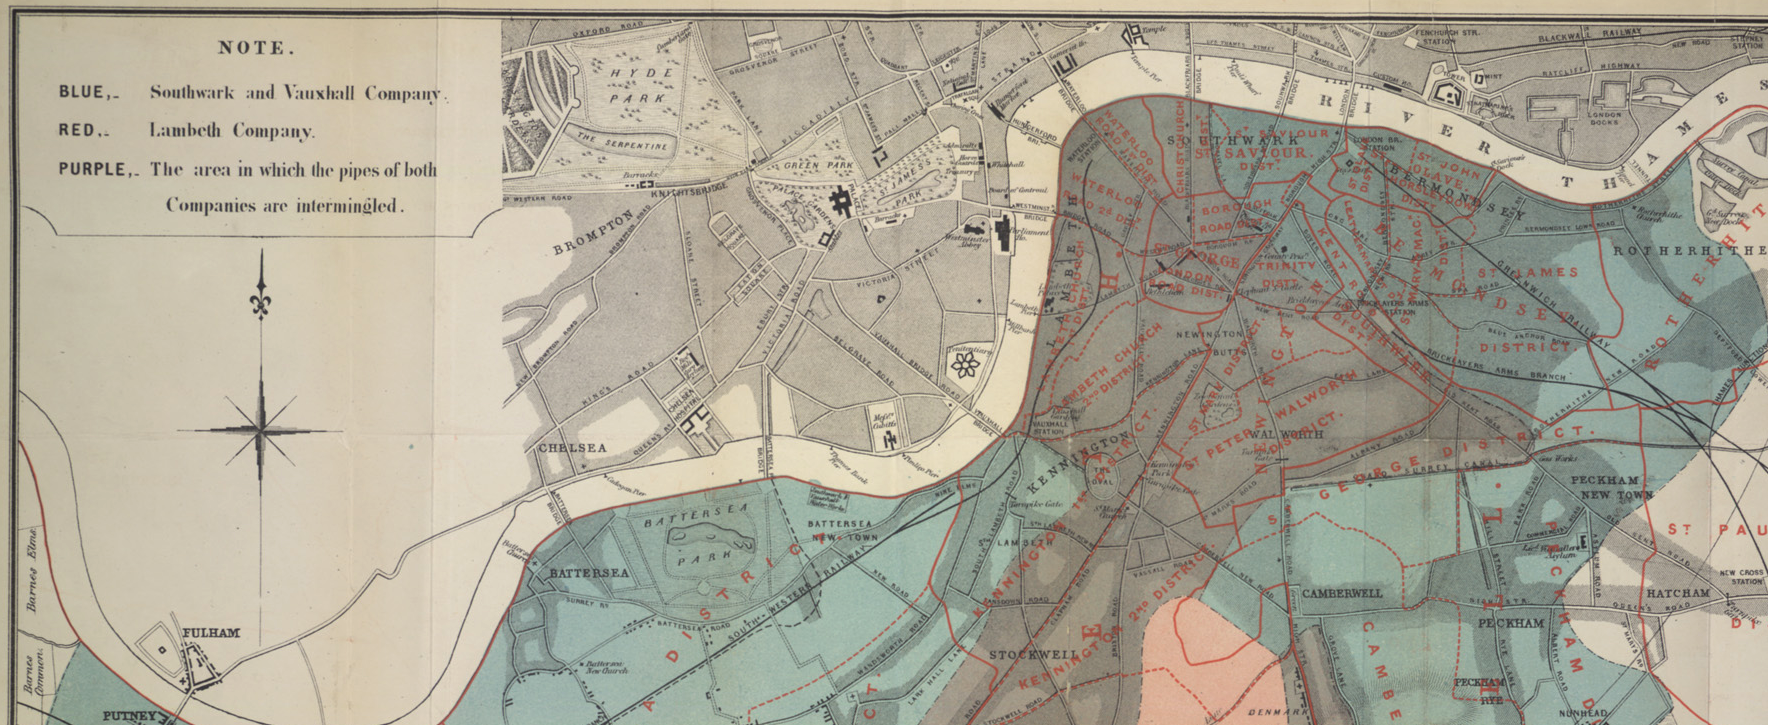
\includegraphics[width = \textwidth]{../img/snow_map}

\begin{itemize}
  \item Probably first use of DiD and natural experiments?
  \item Lambeth Company moved water intake upriver in 1952, Southwark \& Vauxhall Company still got it from downstream
\end{itemize}

\end{frame}
% ----------------------------------------------------

% ----------------------------------------------------
\begin{frame}
\frametitle{Difference-in-differences: Cholera in London}
\centering

\begin{minipage}{0.49\textwidth}\centering
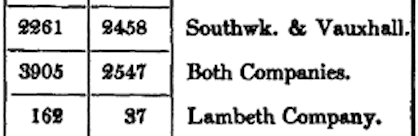
\includegraphics[width = 0.8\textwidth]{../img/snow_table12_zoom}\\\vspace{25pt}
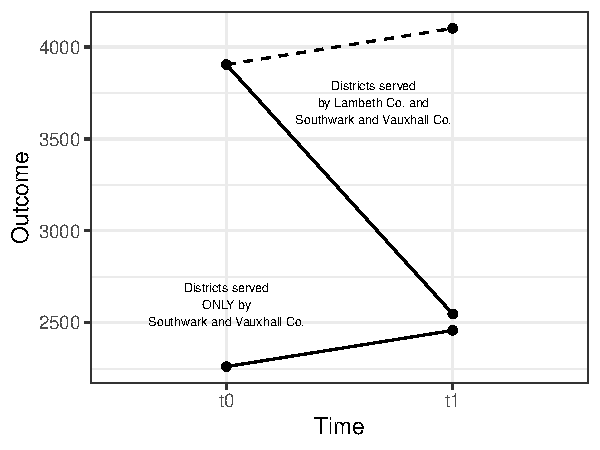
\includegraphics[width = \textwidth]{../img/did_snow}
\end{minipage}\hfill
\begin{minipage}{0.49\textwidth}\centering
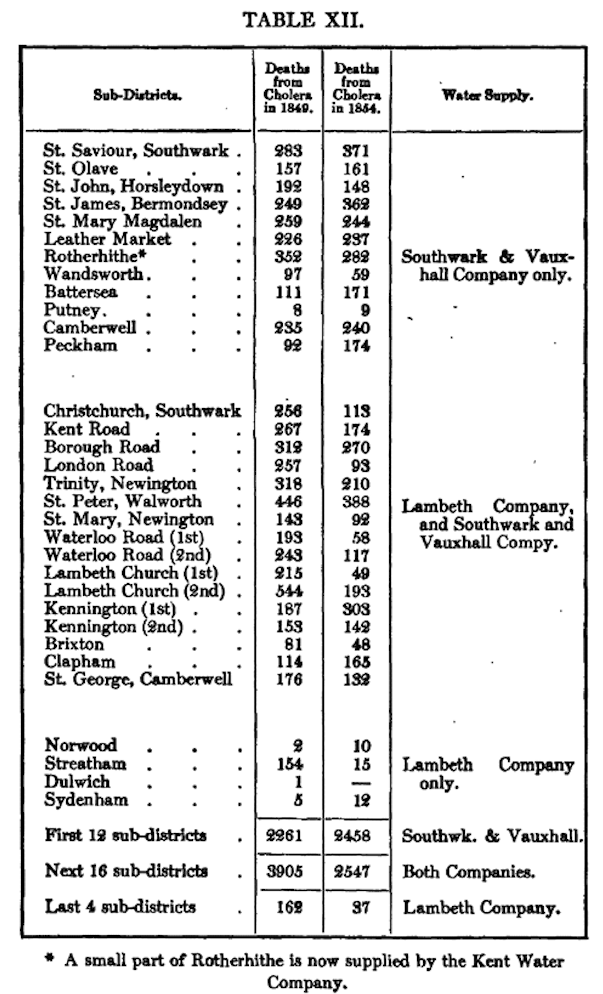
\includegraphics[width = \textwidth]{../img/snow_table12}
\end{minipage}

\end{frame}
% ----------------------------------------------------

% ----------------------------------------------------
\begin{frame}
\frametitle{Difference-in-differences}
\centering

\begin{itemize}
  \item You can estimate this effect just with group means
  \item But it is often easier to use regression, also because you can include controls:
\end{itemize}

\begin{equation}
\begin{split}
    Y_{it} =&  \beta_0 + \beta_1 Treated_{i} + \beta_2 After_{t} +\\
    &\beta_3 (Treated_{i} \times After_{t}) + \beta^\top \mathbf{x}_{i} + \epsilon_{it}
\end{split}
\end{equation}

\begin{itemize}
  \item But why do we need all this?
\end{itemize}

\end{frame}
% ----------------------------------------------------

% ----------------------------------------------------
\begin{frame}
\frametitle{Difference-in-differences}
\centering

\begin{itemize}
  \item Because DiD identification \textbf{depends} on the assumption that the \textbf{control group is a good counterfactual to the treated group}
\end{itemize}


\begin{tikzpicture}
% nodes %
\node (Y) at (2,0){Outcome};
\node (D) at (-2,0){Treatment};
\node (T) at (0,1){Time};
\node (G) at (0,-1){Group};
\node (U) at (0,2){U};
\draw[->] (D) -- (Y);
\draw[->] (T) -- (D);
\draw[->] (T) -- (Y);
\draw[->] (G) -- (Y);
\draw[->] (G) -- (D);
\draw[->, dashed] (U) to [out=0,in=90] (Y);
\draw[->, dashed] (U) to [out=180,in=90] (D);
\end{tikzpicture}


\begin{itemize}
  \item One way to test this is checking if the \textbf{parallel trends assumption} holds (we need data further back in time)
\end{itemize}

\end{frame}
% ----------------------------------------------------

% ----------------------------------------------------
\begin{frame}
\frametitle{DiD example}
\centering

\begin{itemize}
  \item What is the effect of symbolic TJ policies?
  \item \href{https://journals.sagepub.com/doi/full/10.1177/20531680211058550}{journals.sagepub.com/doi/full/10.1177/20531680211058550}
\end{itemize}

\end{frame}
% ----------------------------------------------------

% ----------------------------------------------------
\begin{frame}
\frametitle{DiD example}
\centering

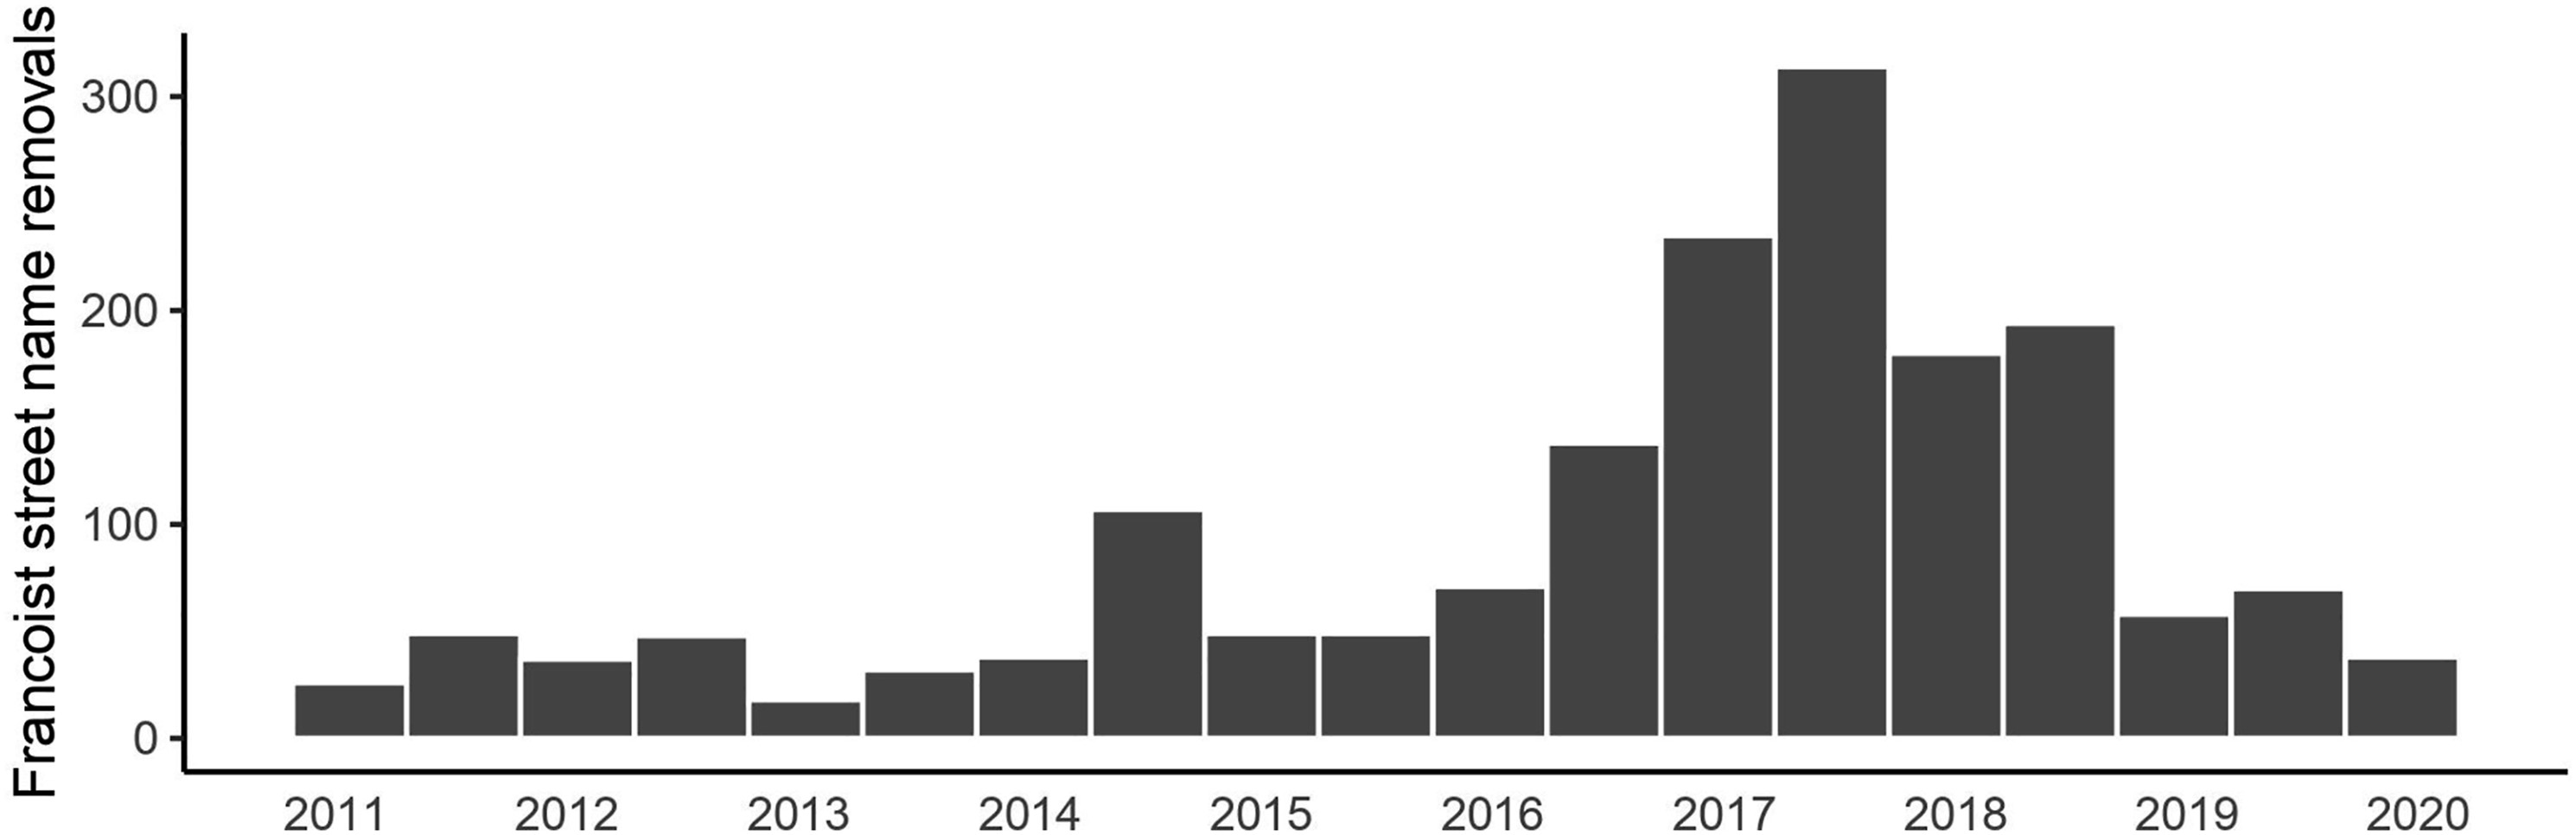
\includegraphics[width = \textwidth]{../img/did_TJ_hist}

\end{frame}
% ----------------------------------------------------

% ----------------------------------------------------
\begin{frame}
\frametitle{DiD example}
\centering

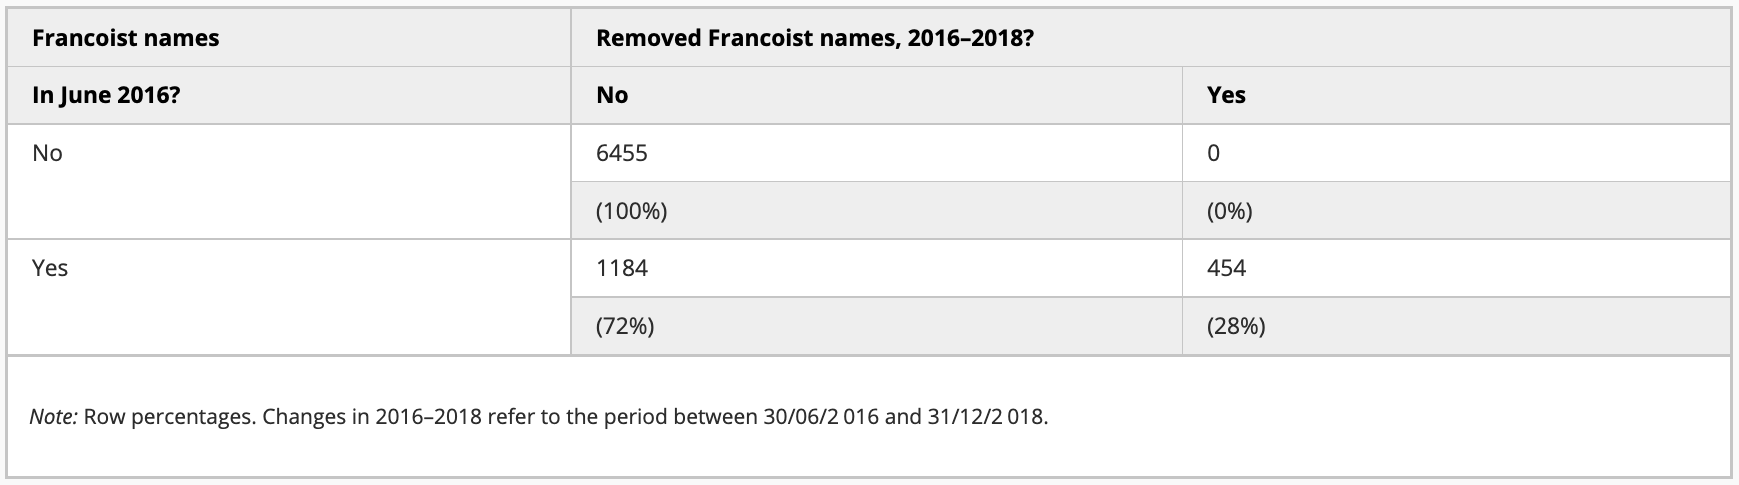
\includegraphics[width = \textwidth]{../img/did_TJ_groups}

\end{frame}
% ----------------------------------------------------


% ----------------------------------------------------
\begin{frame}
\frametitle{DiD example}
\centering

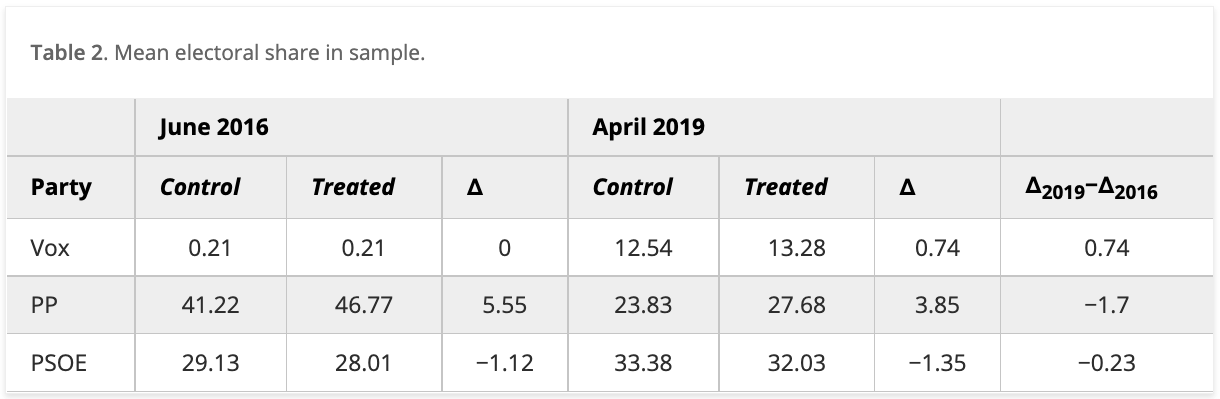
\includegraphics[width = \textwidth]{../img/did_TJ_base}

\end{frame}
% ----------------------------------------------------

% ----------------------------------------------------
\begin{frame}
\frametitle{DiD example}
\centering

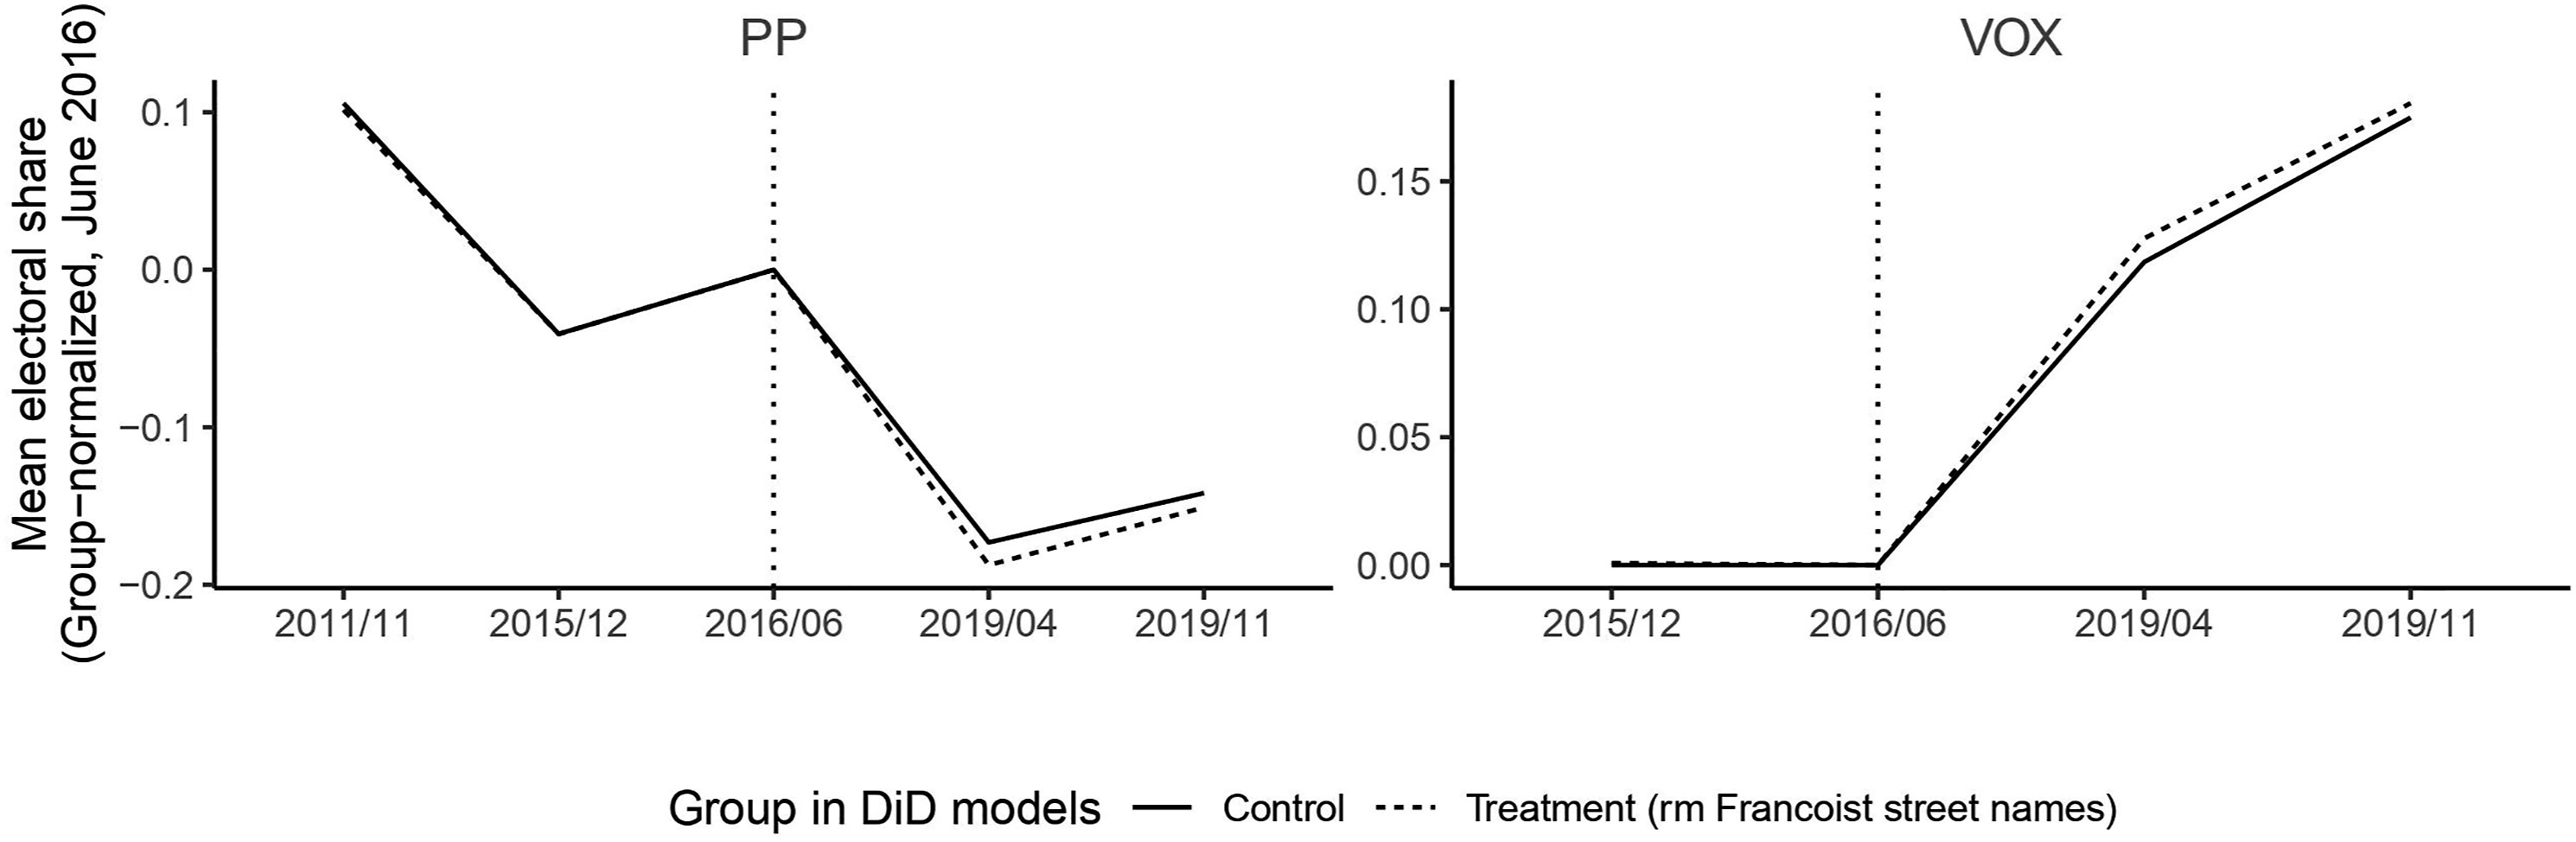
\includegraphics[width = \textwidth]{../img/did_TJ}

\end{frame}
% ----------------------------------------------------

\subsection{Regression discontinuity}

% ----------------------------------------------------
\begin{frame}
\frametitle{Regression discontinuity}
\centering

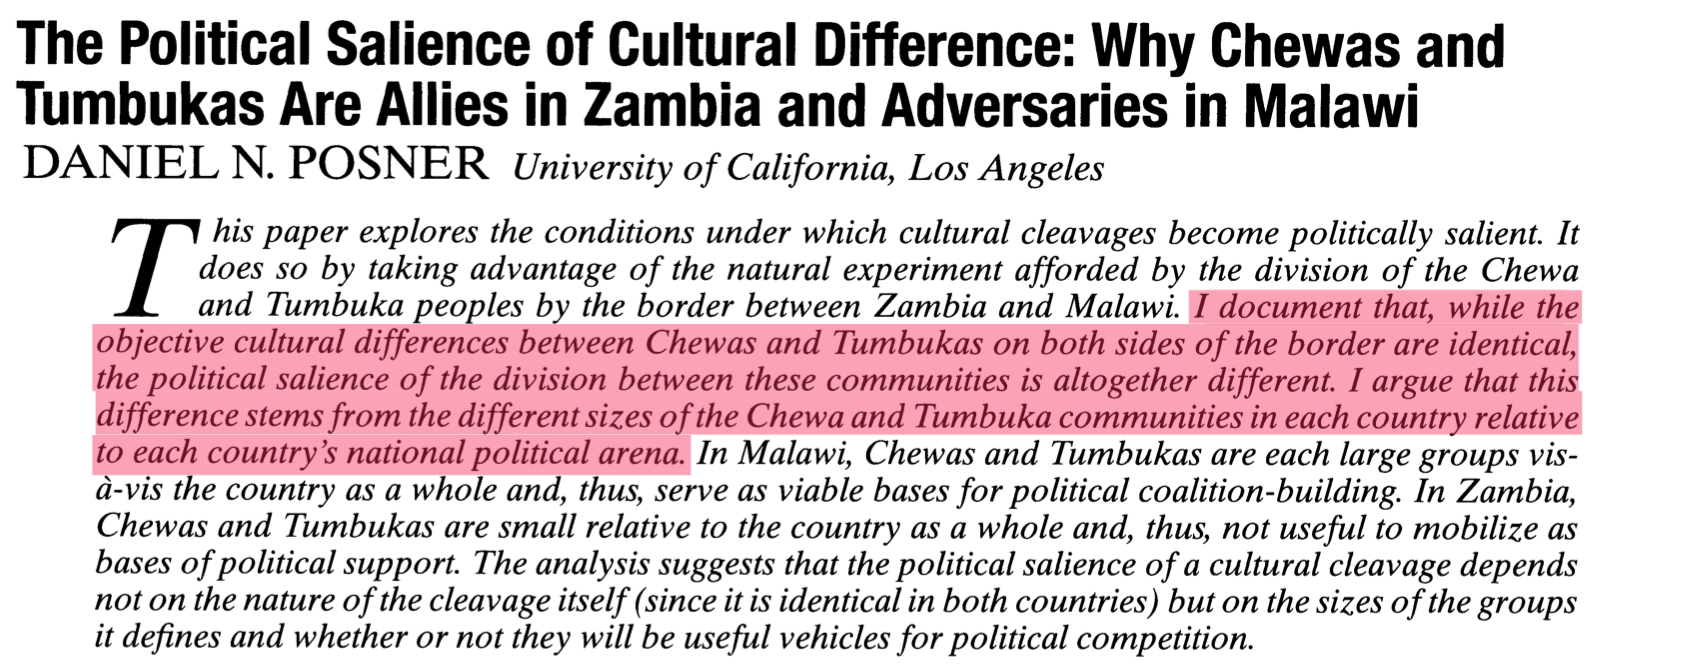
\includegraphics[width = \textwidth]{../img/posner1}

\end{frame}
% ----------------------------------------------------

% ----------------------------------------------------
\begin{frame}
\frametitle{Regression discontinuity}
\centering

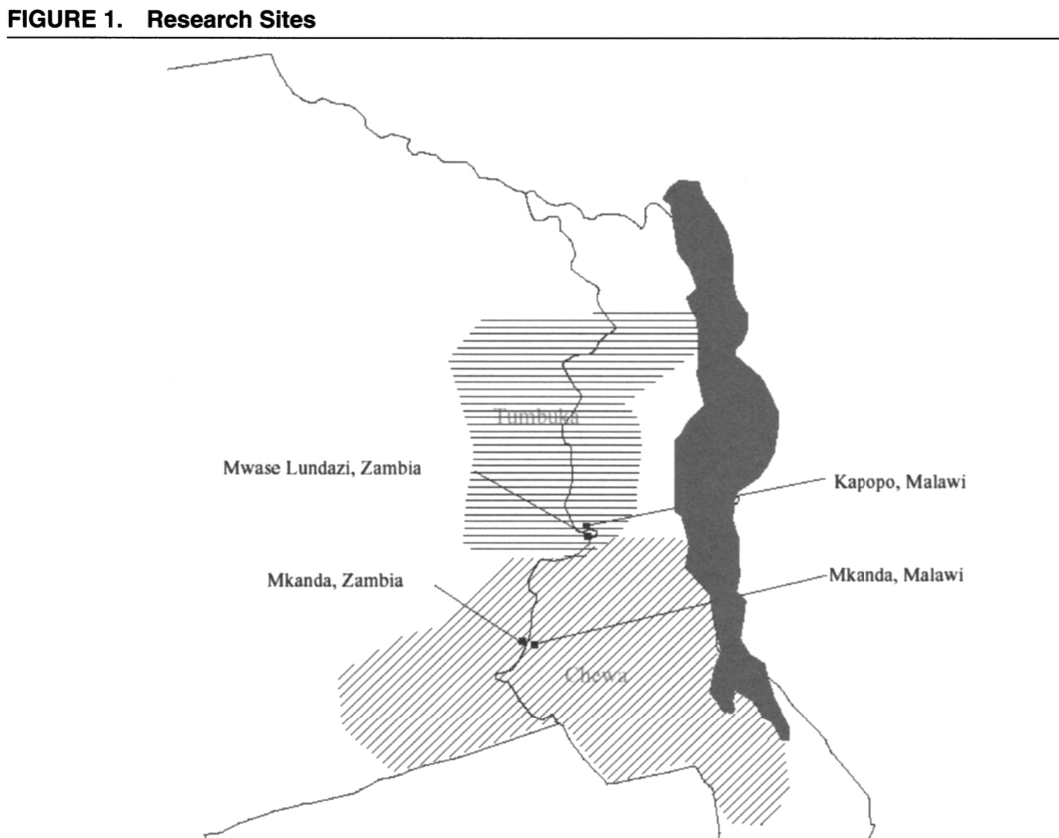
\includegraphics[width = \textwidth]{../img/posner2}

\end{frame}
% ----------------------------------------------------


% ----------------------------------------------------
\begin{frame}
\frametitle{Regression discontinuity}
\centering

\begin{itemize}
  \item RDD works well when assignment into treatment depends on a cutoff along a \textbf{running variable}
  \begin{itemize}
    \item Do incumbent politicians have an electoral advantage? (vote sahre)
    \item What is the effect of being drafted into the military? (birth year)
    \item Effect of national policies in ethnic identification in Africa? (distance to colonial borders)
  \end{itemize}
  \item This is the source of the exogenous variation (or if you will, the natural experiment):
  \begin{itemize}
    \item Although many variables confound the relationships between $X$ and $Y$, nothing should be too different \textit{around the cutoff} between treatment and control groups (local randomization assumption)
    \item Sometimes you look at different \textit{bandwidths} to check this
  \end{itemize}
\end{itemize}

\end{frame}
% ----------------------------------------------------

% ----------------------------------------------------
\begin{frame}
\frametitle{RDD}
\centering

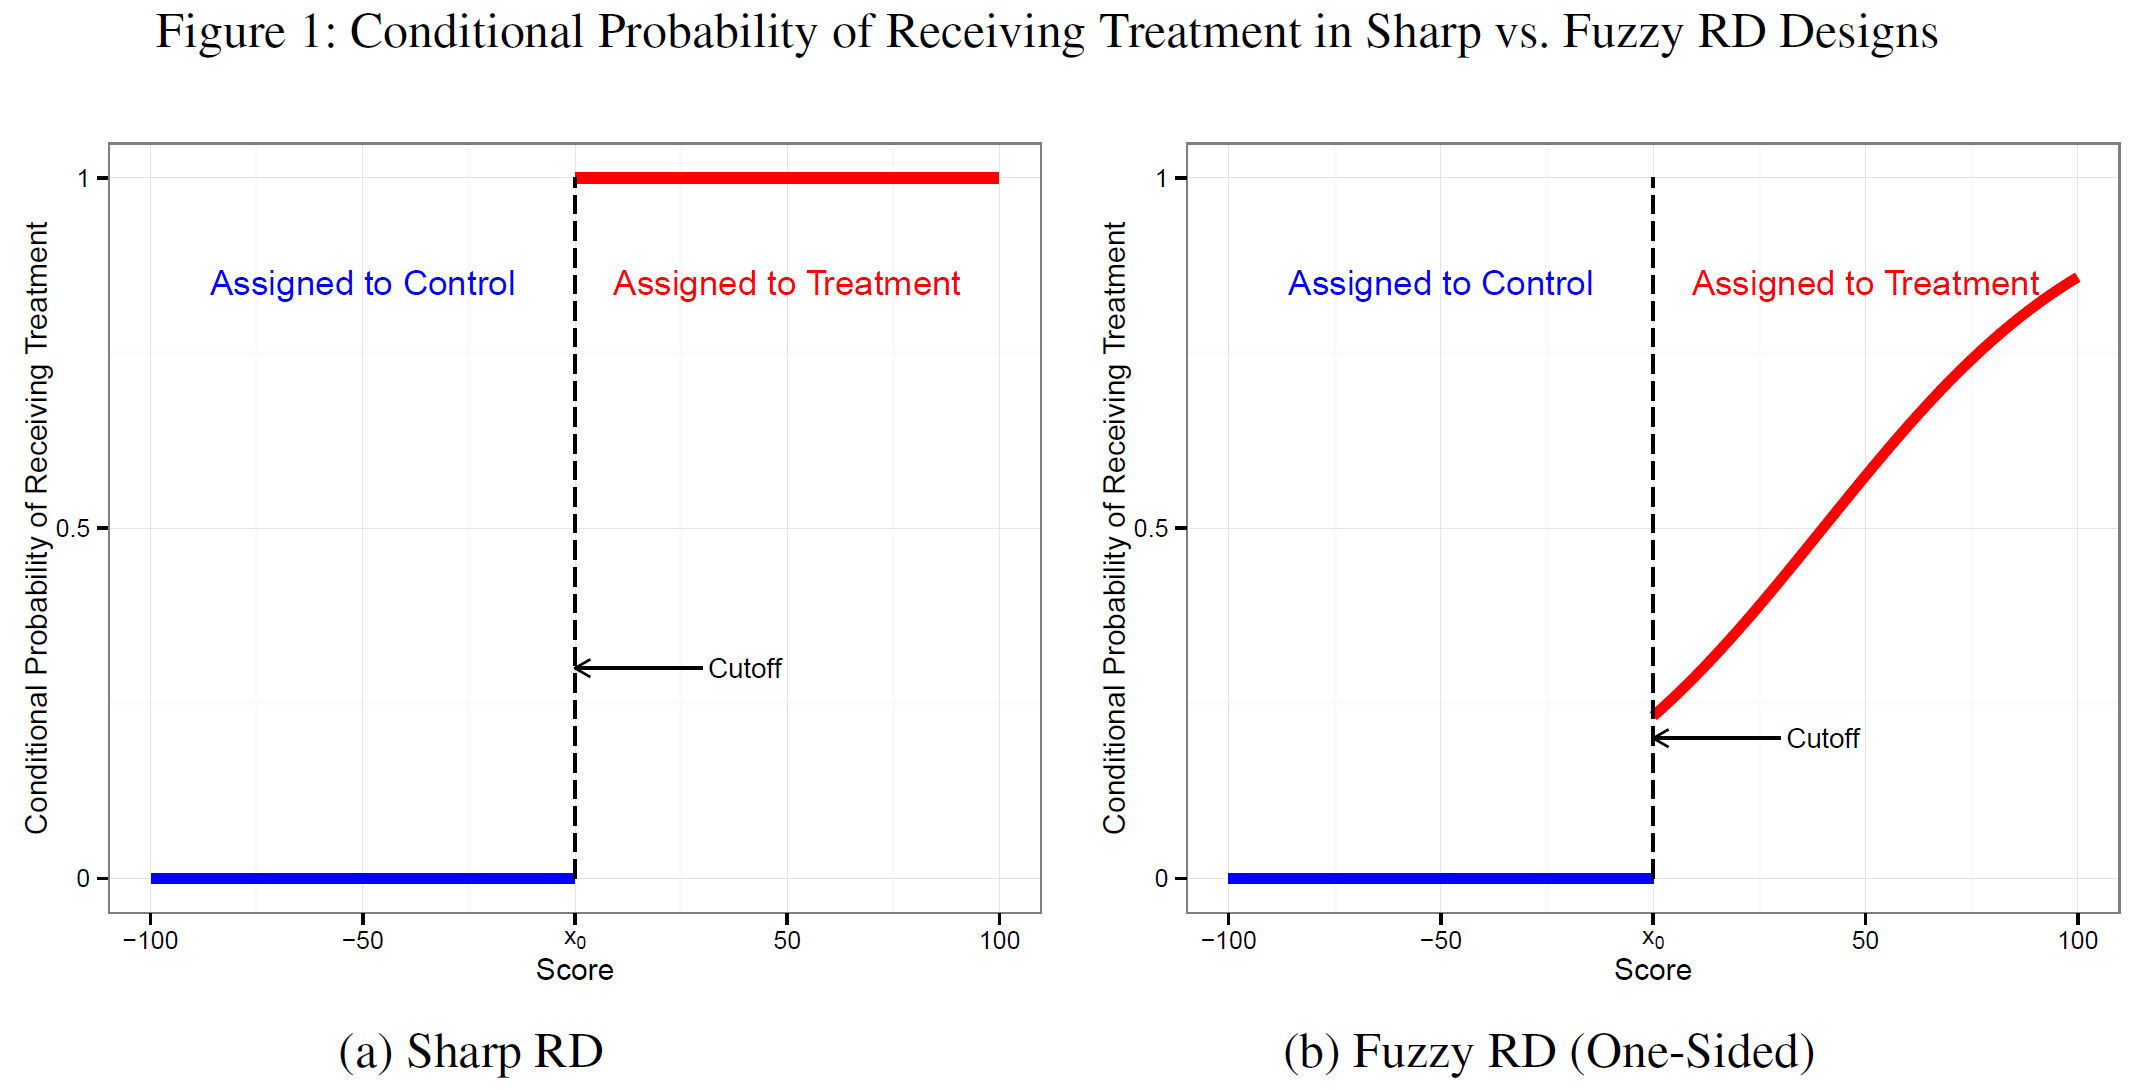
\includegraphics[width = \textwidth]{../img/sharp-fuzzy-rd}

\href{https://bookdown.org/paul/applied-causal-analysis/rddbasics2.html}{\scriptsize https://bookdown.org/paul/applied-causal-analysis/rddbasics2.html}

\end{frame}
% ----------------------------------------------------

% ----------------------------------------------------
\begin{frame}
\frametitle{RDD}
\centering

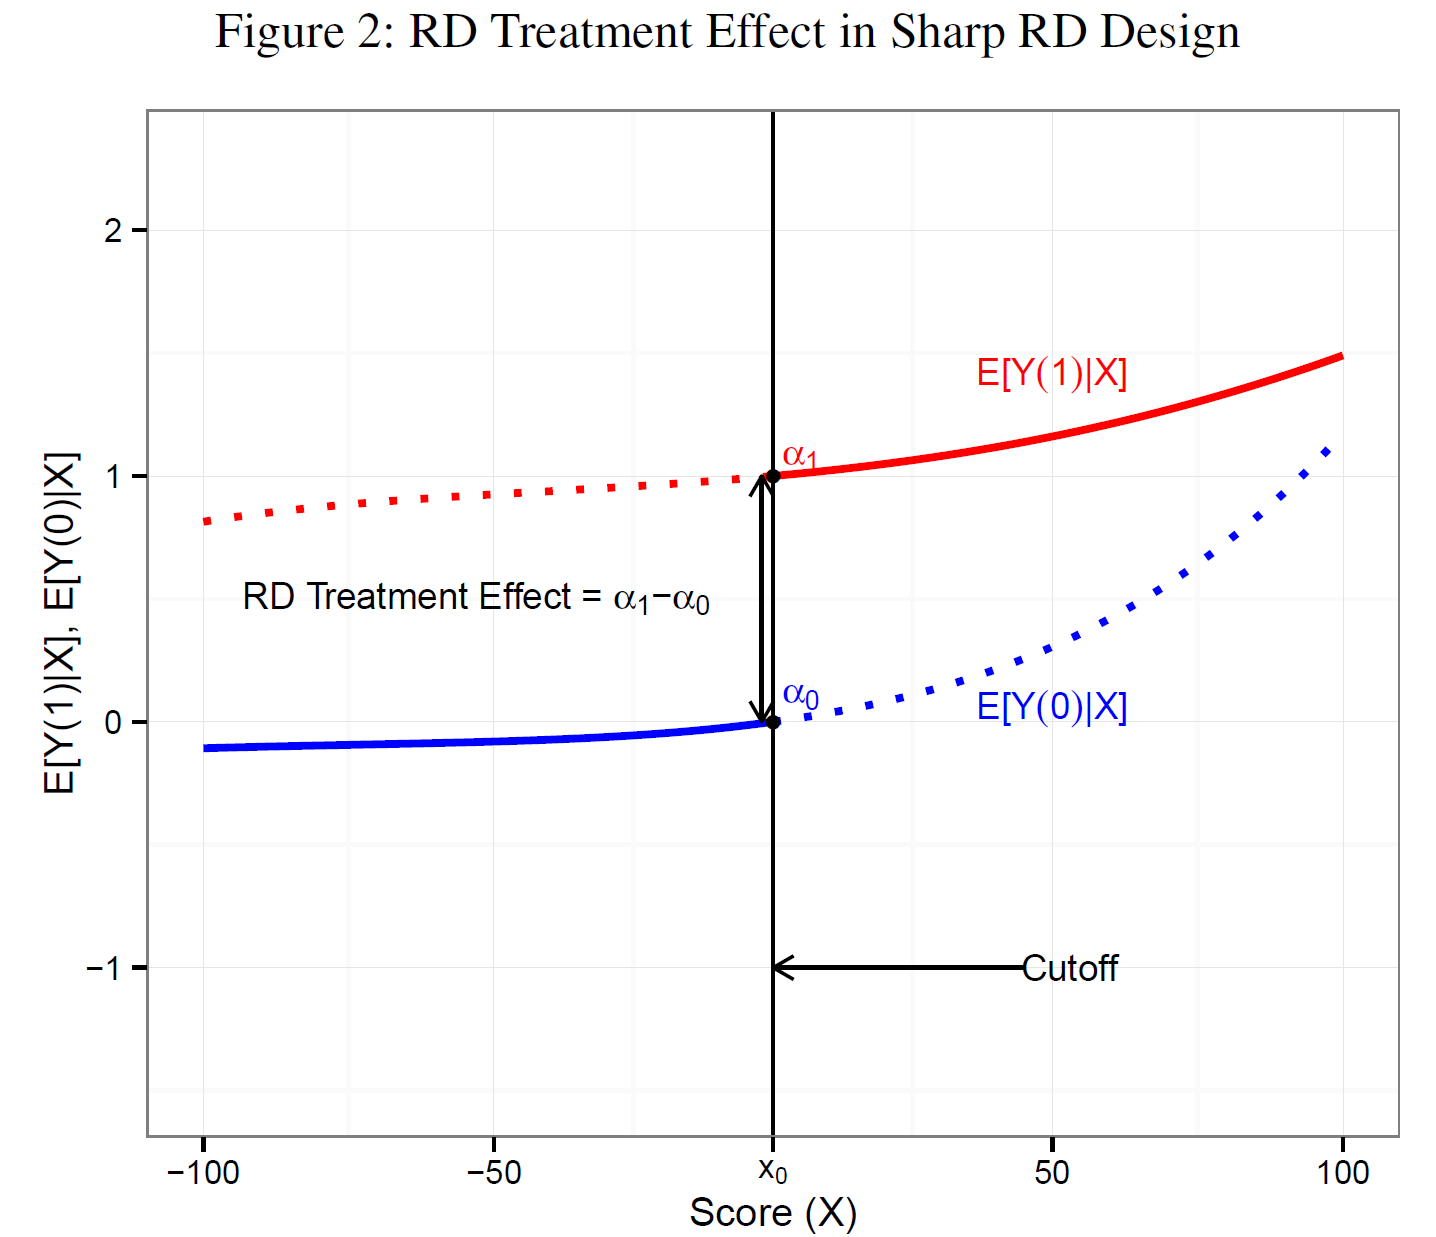
\includegraphics[width = 0.8\textwidth]{../img/rdd_teffect}

\href{https://bookdown.org/paul/applied-causal-analysis/rddbasics3.html}{\scriptsize https://bookdown.org/paul/applied-causal-analysis/rddbasics3.html}

\end{frame}
% ----------------------------------------------------

% ----------------------------------------------------
\begin{frame}
\frametitle{RDD}
\centering

\begin{itemize}
  \item Underlying assumption: other confounders also vary along the running variable, but are independent to the \textit{jump}
\end{itemize}

\vspace{50pt}

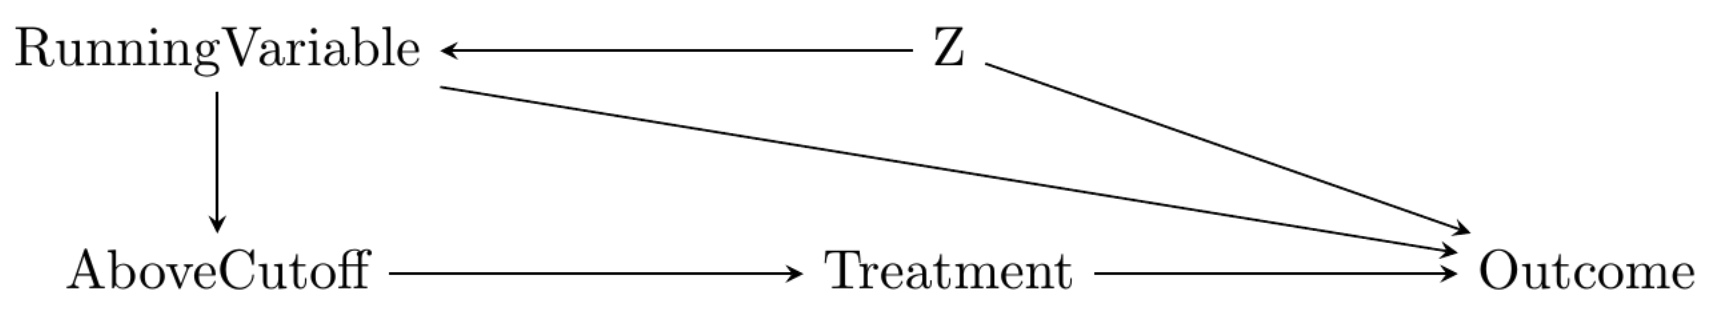
\includegraphics[width = \textwidth]{../img/rdd_dag}

{\scriptsize Huntington-Klein, \textit{The Effect}, p.508}

\end{frame}
% ----------------------------------------------------

% ----------------------------------------------------
\begin{frame}
\frametitle{RDD}
\centering

\begin{itemize}
  \item Underlying assumption: other confounders also vary along the running variable, but are independent to the \textit{jump}
  \item Even if in a \textit{fuzzy} design
\end{itemize}

\vspace{30pt}

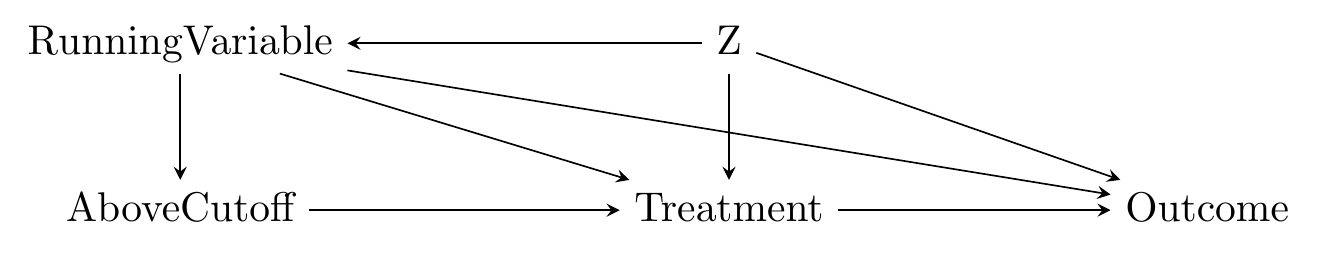
\includegraphics[width = \textwidth]{../img/rdd_dag_fuzzy}

{\scriptsize Huntington-Klein, \textit{The Effect}, p.508}

\end{frame}
% ----------------------------------------------------

% ----------------------------------------------------
\begin{frame}
\frametitle{RDD implementation}
\centering

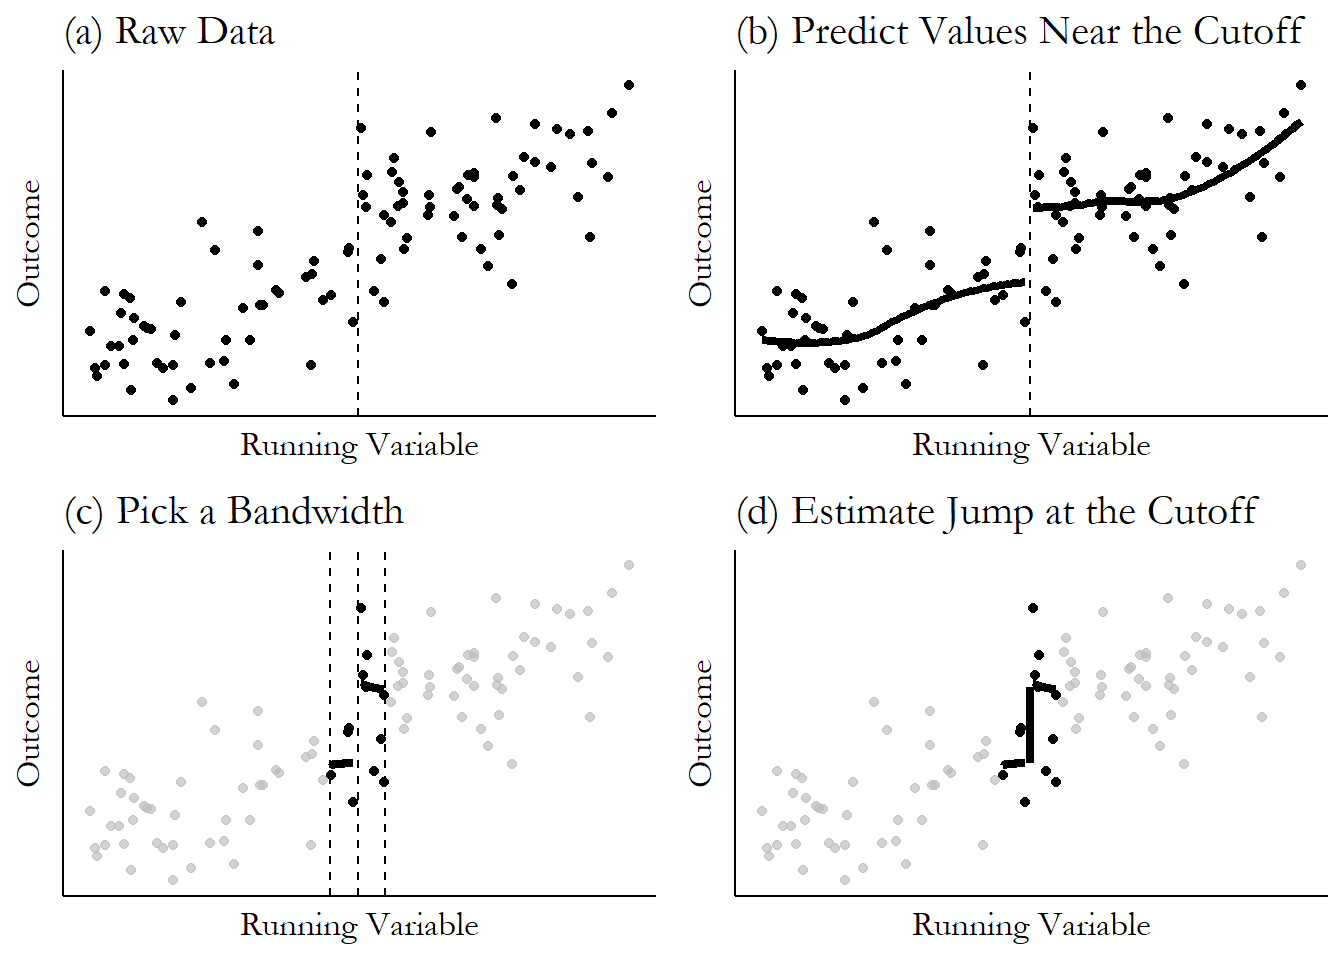
\includegraphics[width = \textwidth]{../img/rdd_procedure}

{\scriptsize Huntington-Klein, \textit{The Effect}, p.509}

\end{frame}
% ----------------------------------------------------

% ----------------------------------------------------
\begin{frame}
\frametitle{RDD and regression}
\centering


\begin{minipage}{0.49\textwidth}\centering
\begin{equation}
\begin{split}
    Y =&  \beta_0 + \beta_{1} Distance +\\
    &\beta_2 Treated +\\
    &\beta_3 (Treated \times Distance) + \beta^\top \mathbf{x}_{i} + \epsilon_{it}
\end{split}
\end{equation}
\end{minipage}\hfill
\begin{minipage}{0.49\textwidth}\centering
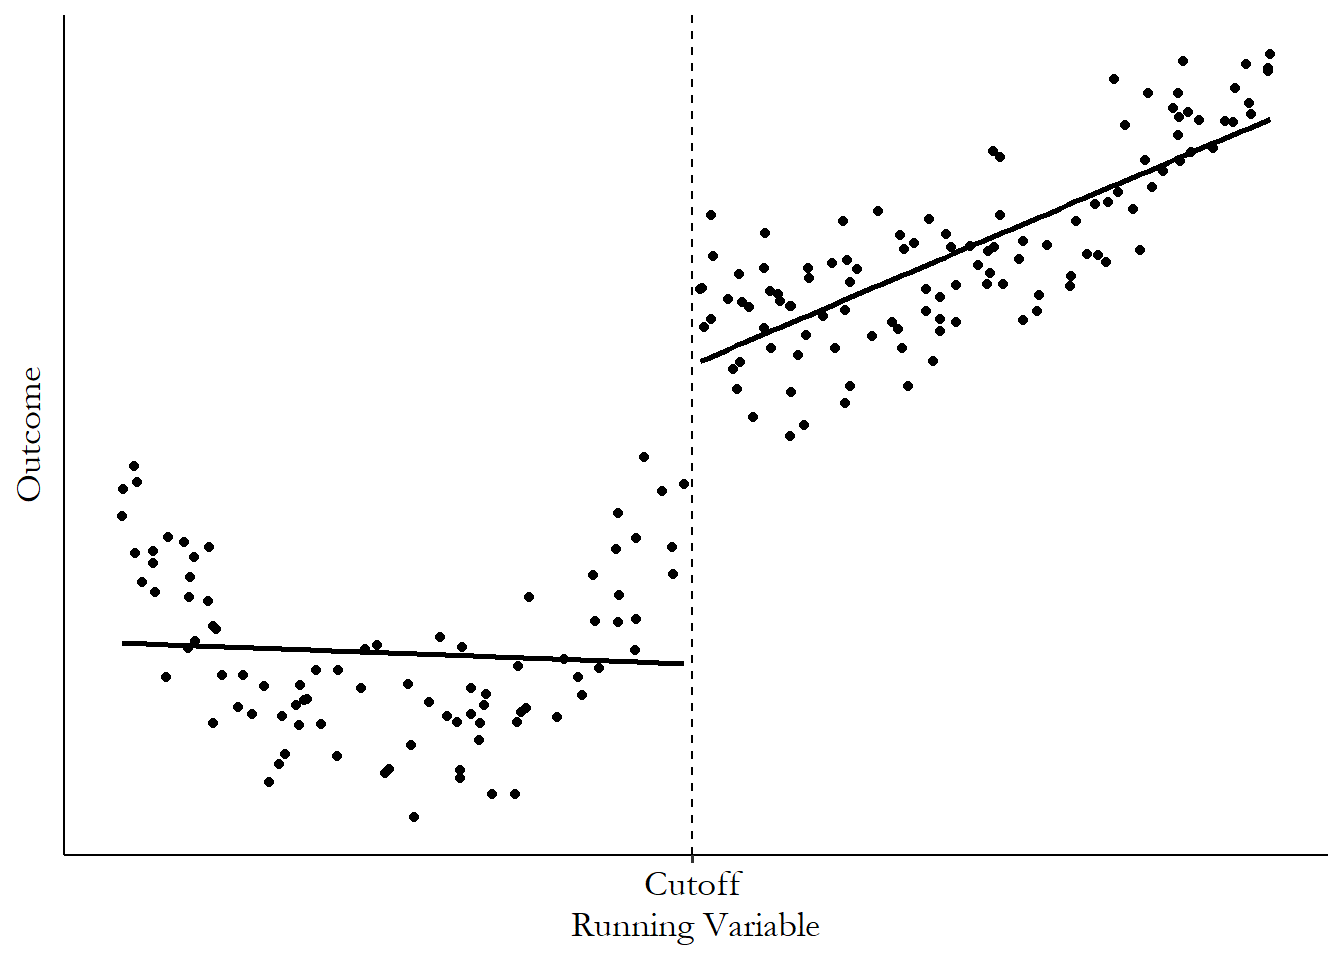
\includegraphics[width = \textwidth]{../img/rdd_lm}
\end{minipage}


\begin{itemize}
  \item But there's no need to use linear regression, other methods available as well
\end{itemize}

\end{frame}
% ----------------------------------------------------


% ----------------------------------------------------
\begin{frame}
\frametitle{Threats to RDD: precise sorting}
\centering

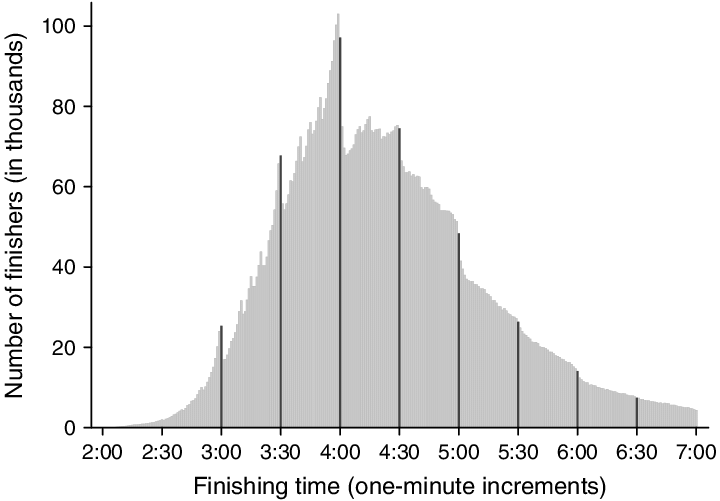
\includegraphics[width = \textwidth]{../img/marathon_finishing_times}

\end{frame}
% ----------------------------------------------------

% ----------------------------------------------------
\begin{frame}
\frametitle{Threats to RDD: cutoff $\leftarrow$ outcome}
\centering

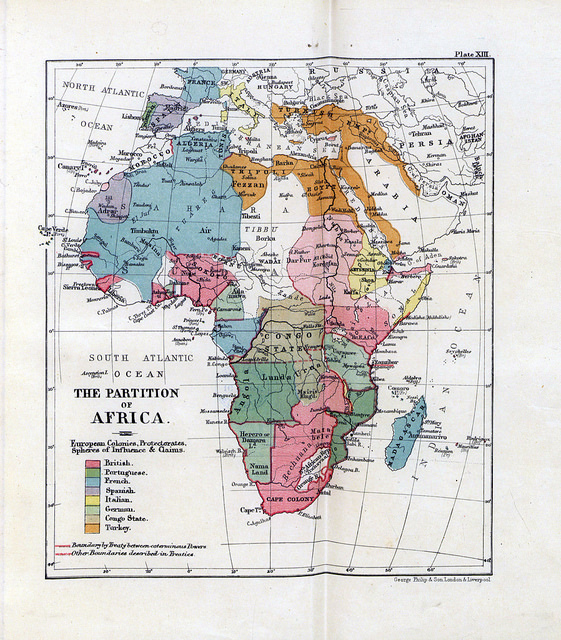
\includegraphics[width = 0.7\textwidth]{../img/partition_africa}

\end{frame}
% ----------------------------------------------------

% ----------------------------------------------------
\begin{frame}
\frametitle{Threats to RDD}
\centering

\begin{tikzpicture}
\node (Y) at (3,0){Outcome};
\node (D) at (0,0){Treatment};
\node (c) at (-3,0){Above cutoff};
\node (r) at (-3,1.5){Running var};
\node (z) at (0,2.5){Z};
\node (U) at (-1,-3){U};
\draw[->] (D) -- (Y);
\draw[->] (c) -- (D);
\draw[->] (r) -- (c);
\draw[->] (z) -- (r);
\draw[->] (z) -- (Y);
\draw[->] (r) -- (Y);
\draw[->, red] (U) -- (Y);
\draw[->, red] (U) -- (c);
\draw[->, red] (c) to [out=330,in=210] (Y);
\end{tikzpicture}

\end{frame}
% ----------------------------------------------------

% ----------------------------------------------------
\begin{frame}
\frametitle{Some extensions \& combinations}
\centering

\begin{itemize}
  \item DiD with multiple treatment periods (units being treated at different times)
  \item Matched DiD
  \item Difference-in-discontinuities
\end{itemize}

\end{frame}
% ----------------------------------------------------

\subsection{Instrumental variables}

% ----------------------------------------------------
\begin{frame}
\frametitle{Instrumental variables}
\centering

\begin{tikzpicture}[every text node part/.style={align=center}, scale = 0.75]
\node (r) at (0,0){\texttt{random}};
\node (y) at (7,0){Y};
\node (x) at (3.5,0){X};
\node (u) at (5,1.5){U};
\draw[->] (r) -- (x);
\draw[->] (x) -- (y);
\draw[->, dashed] (u) -- (y);
\draw[->, dashed] (u) -- (x);
\end{tikzpicture}

\end{frame}
% ----------------------------------------------------

% ----------------------------------------------------
\begin{frame}
\frametitle{Instrumental variables}
\centering

\begin{itemize}
  \item<1-> Find an exogenous source of variation in the treatment variable
  \item<1-> Isolate that variation and use it to identify the causal effect
  \item[]
  \item<2-> Assumptions:
  \item<2-> \textbf{Relevance}: the instrument explains at least some part of the treatment variable
  \item<2-> \textbf{Validity} or \textbf{exclusion restriction}: no back door paths between the instrument and the outcome
\end{itemize}

\end{frame}
% ----------------------------------------------------

% ----------------------------------------------------
\begin{frame}
\frametitle{Instrumental variables}
\centering

\begin{tikzpicture}[every text node part/.style={align=center}, scale = 1]
\node (r) at (0,0){\texttt{random}};
\node (y) at (7,0){Y};
\node (x) at (3.5,0){X};
\node (u) at (5,1.5){U};
\node (z) at (3.5,2.5){Z};
\draw[->] (r) -- (x);
\draw[->] (x) -- (y);
\draw[->, dashed] (u) -- (y);
\draw[->, dashed] (u) -- (x);
\draw[->, dashed, red, thick] (z) to [out=0,in=90] (y);
\draw[->, dashed, red, thick] (z) to [out=180,in=90] (r);
\draw[->, dashed, red, thick] (r) to [out=-30,in=-150] (y);
\end{tikzpicture}

\end{frame}
% ----------------------------------------------------

% ----------------------------------------------------
\begin{frame}
\frametitle{IV threats}
\centering


\includegraphics[width = 0.75\textwidth]{../img/rainfall_conflict}


\end{frame}
% ----------------------------------------------------

% ----------------------------------------------------
\begin{frame}
\frametitle{IV threats}
\centering

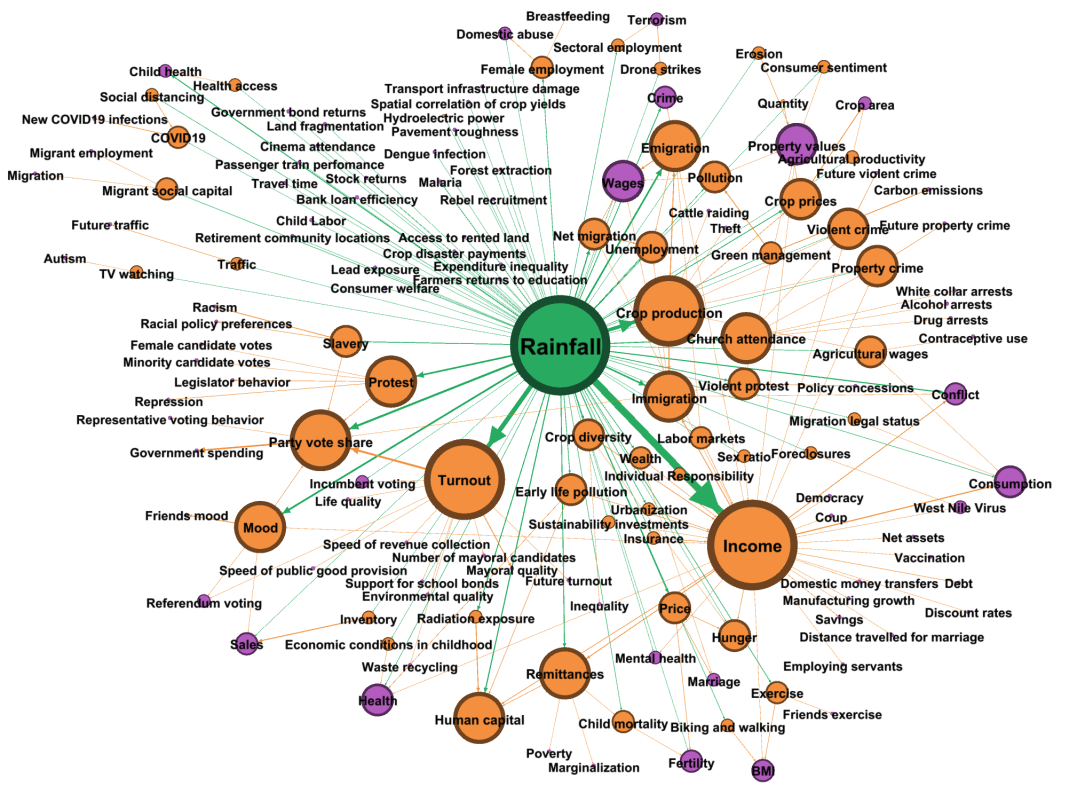
\includegraphics[width = 0.85\textwidth]{../img/rainfall_papers}

{\scriptsize Jonathan Mellon (2022) Rain, Rain, Go Away: 192 Potential Exclusion-Restriction Violations for Studies Using Weather as an Instrumental Variable (\href{https://ssrn.com/abstract=3715610}{https://ssrn.com/abstract=3715610}.)}


\end{frame}
% ----------------------------------------------------



% ----------------------------------------------------
\begin{frame}
\frametitle{How does IV work?}
\centering

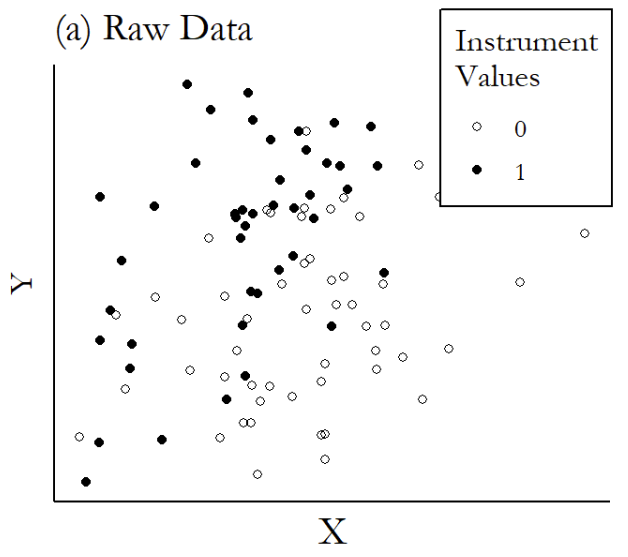
\includegraphics[width = 0.7\textwidth]{../img/ivlogic1}

{\scriptsize (Huntington-Klein, \textit{The Effect}, p 472)}

\end{frame}
% ----------------------------------------------------

% ----------------------------------------------------
\begin{frame}
\frametitle{How does IV work?}
\centering

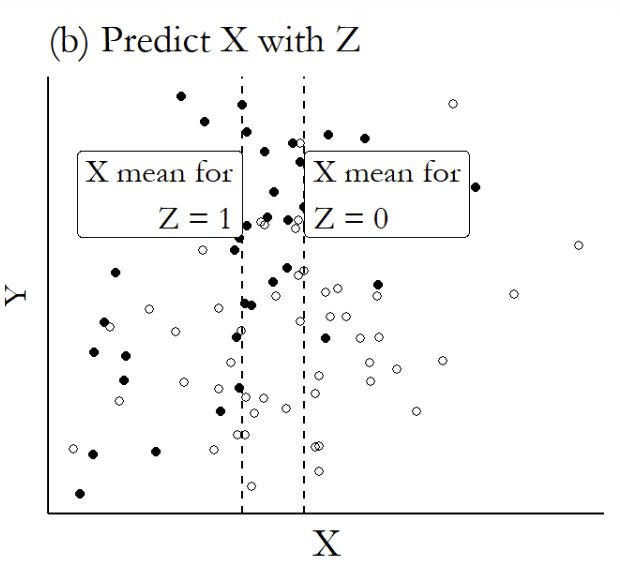
\includegraphics[width = 0.7\textwidth]{../img/ivlogic2}

{\scriptsize (Huntington-Klein, \textit{The Effect}, p 472)}
\end{frame}
% ----------------------------------------------------

% ----------------------------------------------------
\begin{frame}
\frametitle{How does IV work?}
\centering

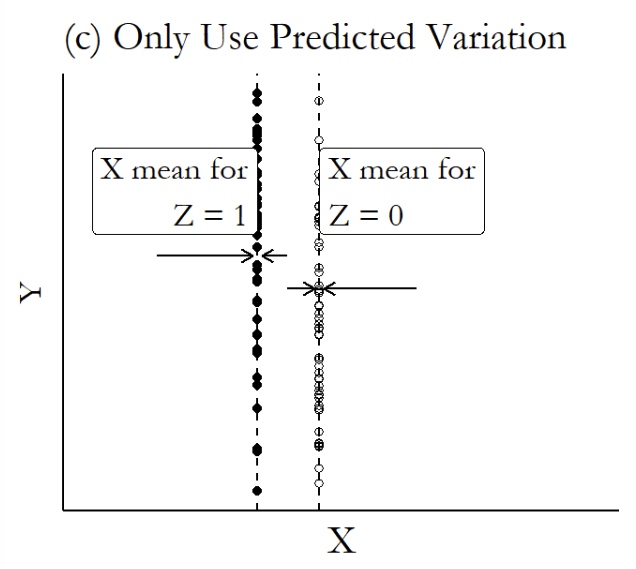
\includegraphics[width = 0.7\textwidth]{../img/ivlogic3}

{\scriptsize (Huntington-Klein, \textit{The Effect}, p 472)}
\end{frame}
% ----------------------------------------------------

% ----------------------------------------------------
\begin{frame}
\frametitle{How does IV work?}
\centering

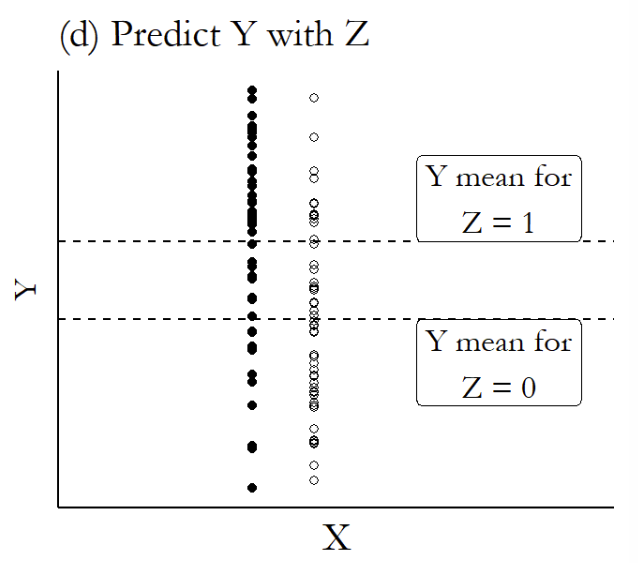
\includegraphics[width = 0.7\textwidth]{../img/ivlogic4}

{\scriptsize (Huntington-Klein, \textit{The Effect}, p 472)}
\end{frame}
% ----------------------------------------------------

% ----------------------------------------------------
\begin{frame}
\frametitle{How does IV work?}
\centering

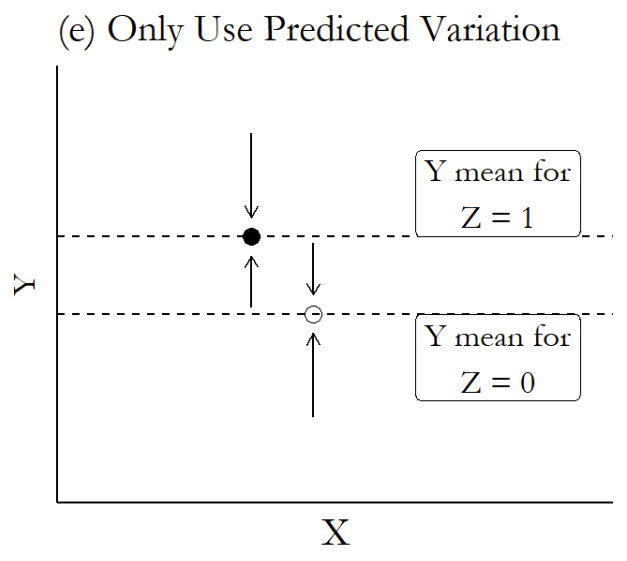
\includegraphics[width = 0.7\textwidth]{../img/ivlogic5}

{\scriptsize (Huntington-Klein, \textit{The Effect}, p 472)}
\end{frame}
% ----------------------------------------------------

% ----------------------------------------------------
\begin{frame}
\frametitle{How does IV work?}
\centering

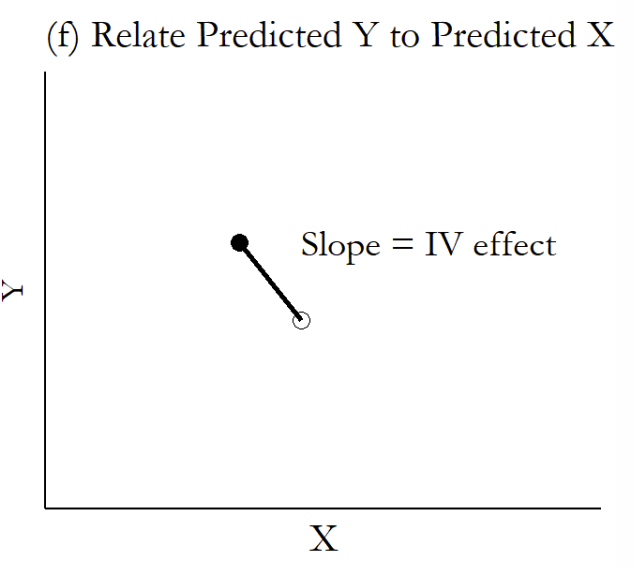
\includegraphics[width = 0.7\textwidth]{../img/ivlogic6}

{\scriptsize (Huntington-Klein, \textit{The Effect}, p 472)}
\end{frame}
% ----------------------------------------------------

% ----------------------------------------------------
\begin{frame}
\frametitle{How does IV work?}
\centering

\begin{itemize}
  \item Usually: two-stage least squares, or \textbf{2SLS}
  \item[1.] Run a `first-stage' regression to predict the treamtnet with the instrument
  \item[2.] Use the predicted values to predict the outcome in the `second-stage'
\end{itemize}

\end{frame}
% ----------------------------------------------------

% ----------------------------------------------------
\begin{frame}
\frametitle{Alternative approaches to IV: build your own}
\centering


\includegraphics[width = 0.8\textwidth]{../img/carl1}

\end{frame}
% ----------------------------------------------------

% ----------------------------------------------------
\begin{frame}
\frametitle{Alternative approaches to IV: build your own}
\centering

\includegraphics[width = \textwidth]{../img/carl9}

\end{frame}
% ----------------------------------------------------

% ----------------------------------------------------
\begin{frame}
\frametitle{Alternative approaches to IV: build your own}
\centering

\includegraphics[width = \textwidth]{../img/carl10}

\end{frame}
% ----------------------------------------------------

% ====================================================
\end{document}
